% ============================================================================
%  Modelo completo del Segway con patas extensibles
%  Documento maestro: ata los cuatro PDF que ya existian y agrega los capitulos
%  del pendulo invertido, el motor, el LQR y Simulink.
%
%  Compilar DOS veces (por el indice) desde esta carpeta:
%     pdflatex -interaction=nonstopmode modelo_del_segway.tex
%  Requiere pdfpages y tcolorbox.
% ============================================================================
\documentclass[11pt,a4paper]{report}
\usepackage[utf8]{inputenc}
\usepackage[T1]{fontenc}
\usepackage[spanish,es-noshorthands]{babel}
\usepackage[margin=2.3cm]{geometry}
\usepackage{amsmath,amssymb}
\usepackage{graphicx}
\usepackage{booktabs}
\usepackage{xcolor}
\usepackage{tcolorbox}
\usepackage{pdfpages}
\usepackage{enumitem}
\usepackage{caption}
\usepackage[colorlinks=true,linkcolor=blue!50!black,urlcolor=blue!50!black,
            citecolor=blue!50!black]{hyperref}

\graphicspath{{../../modelado/}{../../modelado/cinematica/}{../../modelado/dcl/}%
              {../../modelado/dinamica/}{../../modelado/geometria/}%
              {../../modelado/planta/pendulo_invertido/}%
              {../../modelado/planta/pendulo_invertido/diagramas/}%
              {../../simulacion/pendulo_invertido/resultados/}}

\setlength{\parskip}{5pt}
\setlength{\parindent}{0pt}
\captionsetup{font=small,labelfont=bf}

\definecolor{azulp}{RGB}{31,95,168}
\definecolor{verdep}{RGB}{27,94,32}
\definecolor{rojop}{RGB}{198,40,40}
\definecolor{naranjap}{RGB}{217,83,30}

\newtcolorbox{idea}{colback=azulp!6,colframe=azulp,boxrule=0.9pt,
  left=7pt,right=7pt,top=6pt,bottom=6pt,arc=2pt,
  fonttitle=\bfseries,title=La idea}
\newtcolorbox{ojo}{colback=rojop!5,colframe=rojop,boxrule=0.9pt,
  left=7pt,right=7pt,top=6pt,bottom=6pt,arc=2pt,
  fonttitle=\bfseries,title=Ojo con esto}
\newtcolorbox{medido}{colback=verdep!5,colframe=verdep,boxrule=0.9pt,
  left=7pt,right=7pt,top=6pt,bottom=6pt,arc=2pt,
  fonttitle=\bfseries,title=Lo que está medido y lo que no}

\newcommand{\dd}{\mathrm{d}}
\newcommand{\ud}[1]{\,\mathrm{#1}}

\title{\vspace{-1.5cm}\Huge El modelo del Segway con patas extensibles\\[10pt]
\large De la geometría de la pata al controlador que lo mantiene parado\\[18pt]
\normalsize Documento único: ata los cuatro informes que ya existían y agrega\\
el péndulo invertido, el motor, el LQR y la simulación en Simulink}
\author{Grupo 4 --- Robótica II, Facultad de Ingeniería, UNCUYO\\[4pt]
\small Joaquín Calderón \quad\textbullet\quad Francisco Castel \quad\textbullet\quad Matías Armani}
\date{21 de octubre de 2026}

\begin{document}
\maketitle

\begin{idea}
Este documento explica, de abajo hacia arriba, cómo está modelado el robot y por qué
cada pieza del modelo es como es. No supone que el lector haya seguido el proyecto.
Las cuentas largas están en los apéndices, que son los informes originales; los capítulos
de adelante cuentan la historia y dan los números que importan.
\end{idea}

\vspace{4pt}
{\large\bfseries Cómo leer esto}

\begin{center}
\begin{tabular}{@{}p{4.3cm}p{10.4cm}@{}}
\toprule
\textbf{Si querés\ldots} & \textbf{andá a\ldots} \\
\midrule
entender el robot en diez minutos & capítulos \ref{cap:mapa2} y \ref{cap:pend} \\
dimensionar el servo & capítulo \ref{cap:din} y apéndices \ref{ap:dcl} y \ref{ap:dinres} \\
entender el control & capítulos \ref{cap:motor} y \ref{cap:lqr} \\
correr la simulación & capítulo \ref{cap:simulink} \\
saber si mover las patas rompe algo & capítulo \ref{cap:patasmov} \\
saber qué no está medido & capítulo \ref{cap:falta} \\
ver las cuentas completas & los apéndices, que son los informes originales \\
\bottomrule
\end{tabular}
\end{center}

Cada capítulo arranca con un recuadro azul con la idea en una o dos frases. Los recuadros
rojos marcan trampas donde ya nos equivocamos una vez, y los verdes separan lo medido de lo
supuesto, que en este proyecto es la distinción más importante de todas.

\tableofcontents

% ===========================================================================
\chapter{El mapa: qué hay que modelar y por qué}
% ===========================================================================

\section{Qué es el robot}

Un Segway con dos ruedas y, entre cada rueda y la cabina, una \textbf{pata extensible}: un
mecanismo de cuatro barras movido por un servo, que sube y baja el cuerpo. O sea, dos cosas
que a primera vista no se parecen en nada:

\begin{itemize}[leftmargin=1.5em]
\item un \textbf{péndulo invertido sobre ruedas}, que se cae solo y hay que sostenerlo
      moviendo las ruedas;
\item dos \textbf{patas} de un grado de libertad, que cambian la altura del cuerpo.
\end{itemize}

\section{Por qué hacen falta dos modelos y no uno}

Porque son dos problemas con escalas de tiempo distintas, y eso permite separarlos.

El péndulo invertido se cae rápido: sin control, la inclinación se duplica cada
\textbf{94 milisegundos}. Las patas, en cambio, se mueven en segundos. Cuando algo es diez
o veinte veces más lento que otra cosa, se puede modelar cada uno como si el otro estuviera
quieto, y revisar después que el acoplamiento no arruine nada. Eso es exactamente lo que hace
este documento:

\begin{enumerate}[leftmargin=1.6em]
\item \textbf{La pata sola} (capítulos \ref{cap:cin} y \ref{cap:din}), para dimensionar el
      servo y entender qué pasa al aterrizar. Acá la cabina está quieta o sube y baja, pero
      no se cae: hay un solo grado de libertad, el ángulo $\theta$ del servo.
\item \textbf{El péndulo invertido} (capítulo \ref{cap:pend}), con las \emph{patas
      congeladas} en una postura. Acá el grado de libertad de la pata desaparece y quedan
      dos: avance $x$ e inclinación $\varphi$. Es la planta que se controla.
\item \textbf{El acoplamiento} (capítulo \ref{cap:patasmov}), que revisa qué pasa cuando las
      patas sí se mueven mientras el robot se equilibra.
\end{enumerate}

\begin{ojo}
Separar los modelos es una decisión, no una verdad. Vale mientras las patas se muevan despacio
comparado con el equilibrio. El capítulo \ref{cap:patasmov} comprueba que vale, y dice cuál es
el precio.
\end{ojo}

% ===========================================================================
\chapter{El robot que existe hoy}\label{cap:mapa2}
% ===========================================================================

\begin{idea}
Todo el modelo sale de un solo archivo de parámetros. Si un número cambia ahí, cambia en los
cálculos, en las figuras y en los PDF. Eso evita que cada integrante trabaje con un robot
distinto, que es lo que pasaba antes.
\end{idea}

\section{La geometría de la pata}

Segunda iteración del CAD, barras a escala 80, medidas sobre los archivos STEP del 14/9/2026.

\begin{center}
\begin{tabular}{@{}llr@{}}
\toprule
\textbf{Símbolo} & \textbf{Qué es} & \textbf{Valor} \\
\midrule
$AB$ & bancada: del eje del servo al pivote fijo & 80{,}0 mm a $45^\circ$ \\
$AD$ & manivela, la que mueve el servo & 112{,}0 mm \\
$BC$ & balancín & 108{,}0 mm \\
$CD$ & lado corto del acoplador & 40{,}8 mm \\
$DP$ & del acoplador al eje de la rueda & 112{,}0 mm \\
$\delta$ & ángulo del acoplador en $D$, de $D\!\to\!C$ a $D\!\to\!P$ & $164^\circ$ \\
$R_w$ & radio de la rueda & 40 mm \\
$\theta$ & ángulo de $AD$ bajo la horizontal & $10^\circ$ a $40^\circ$ \\
\bottomrule
\end{tabular}
\end{center}

$\theta$ es la coordenada de todo el mecanismo: con $\theta$ queda determinada la posición de
cada barra. $\theta = 10^\circ$ es la pata plegada y $\theta = 40^\circ$ la estirada. El ángulo
absoluto que se le manda al servo es $360^\circ - \theta$.

\begin{center}
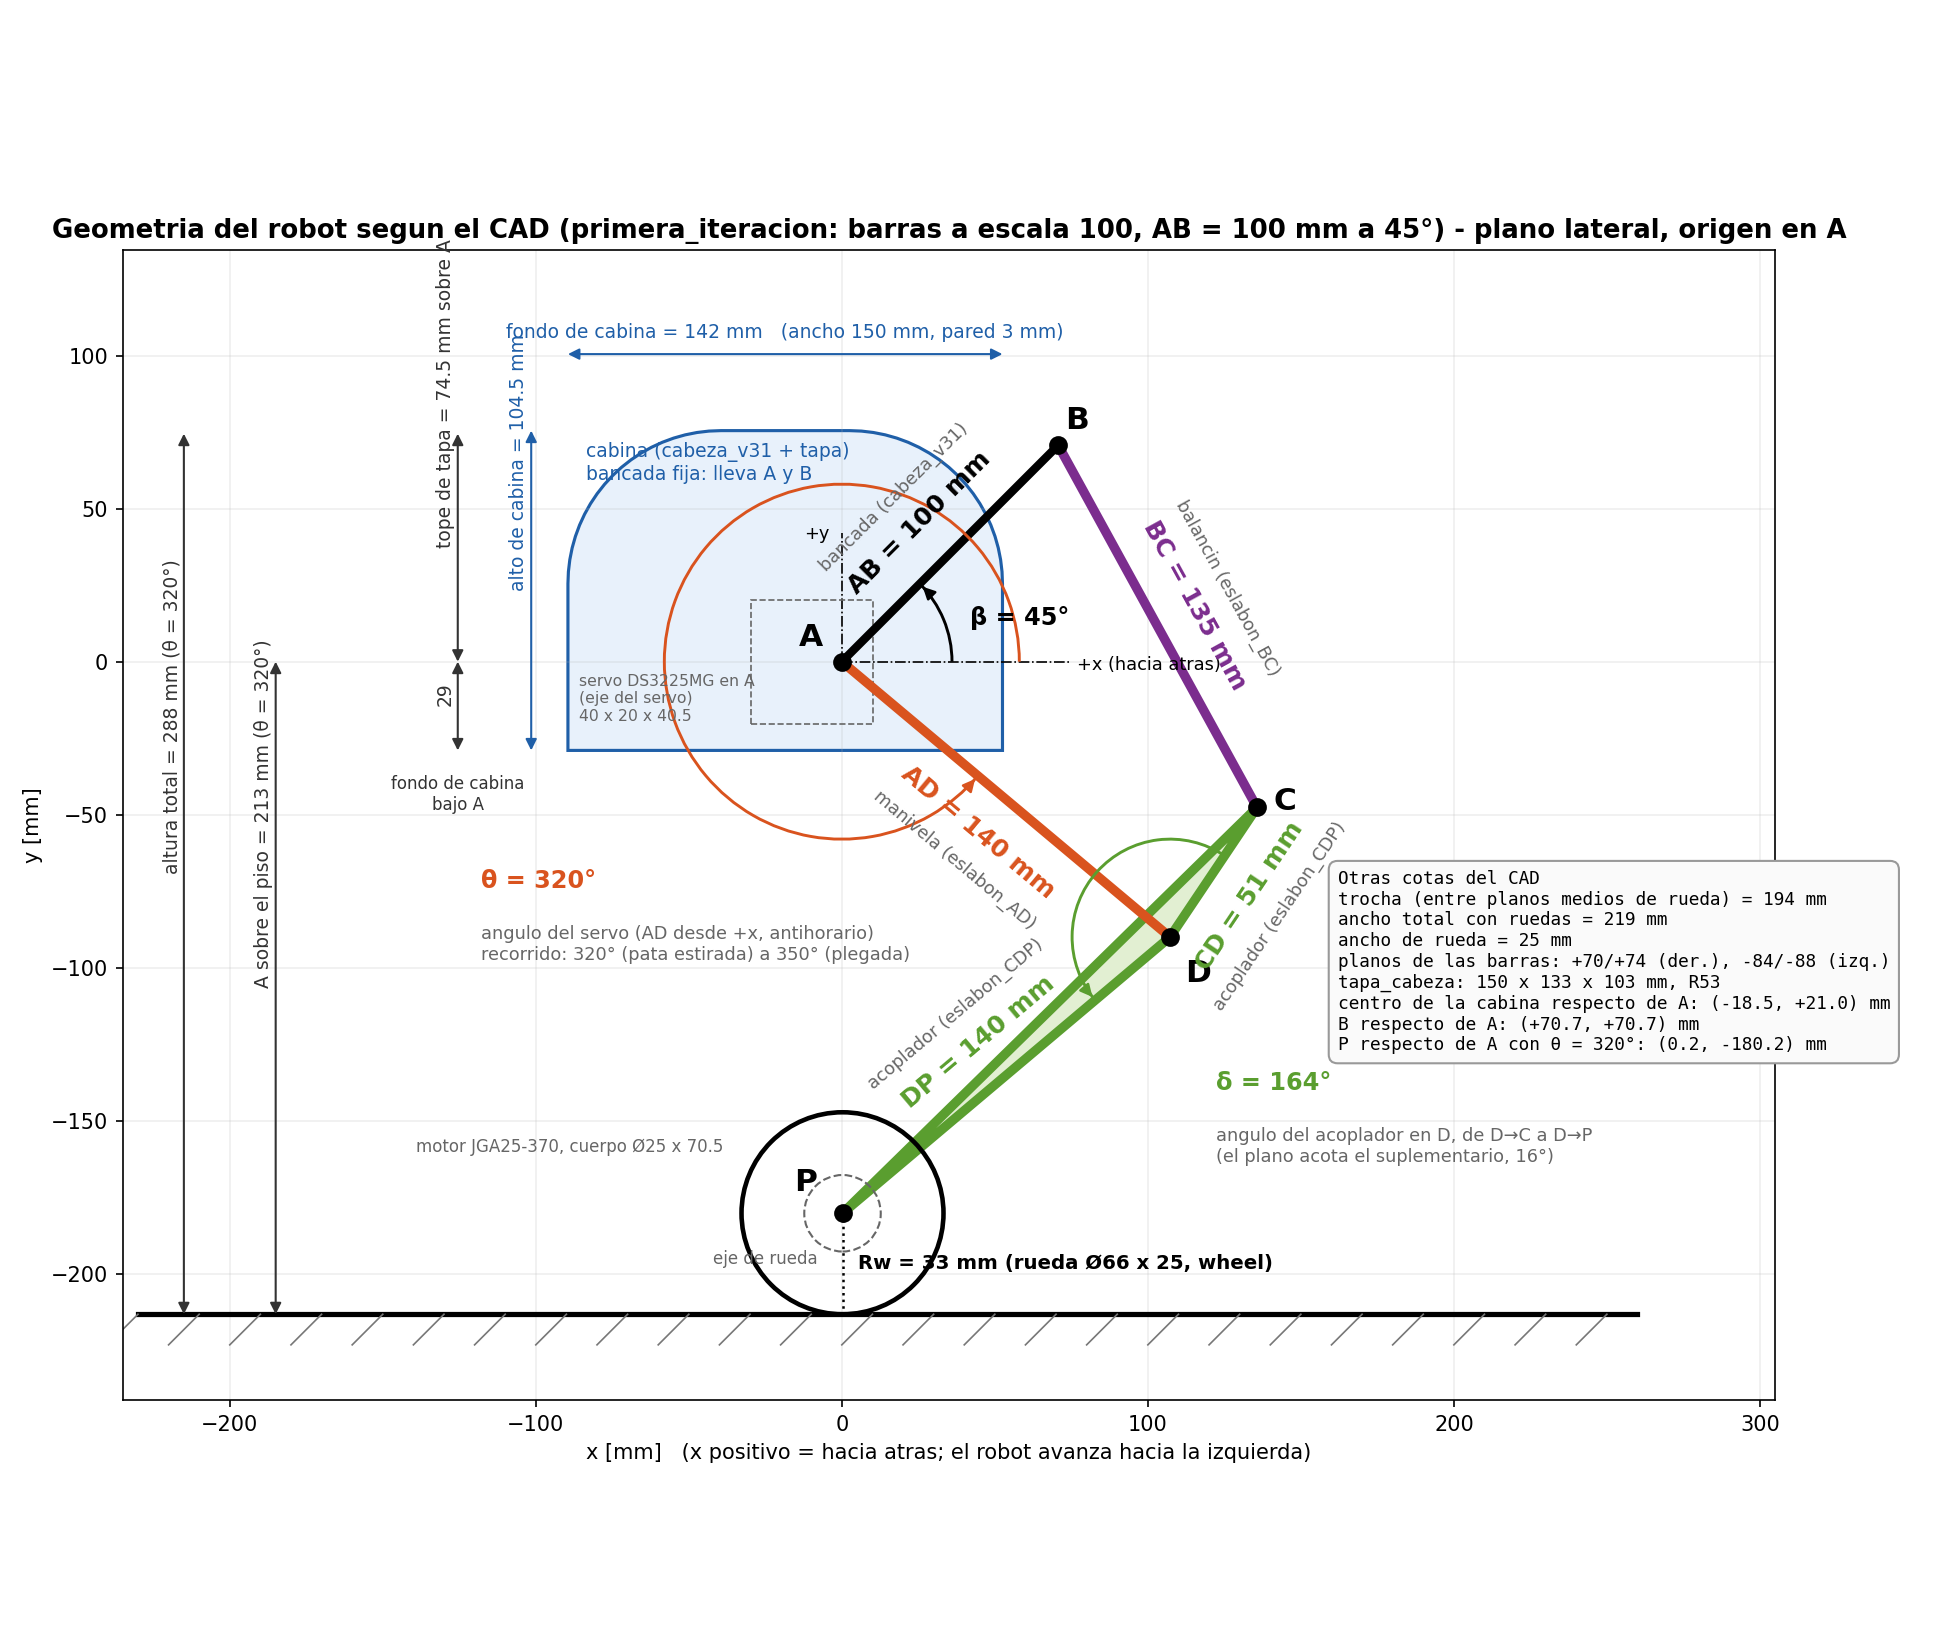
\includegraphics[width=0.93\textwidth]{geometria_robot.png}
\captionof{figure}{El robot con la pata en su postura media. Los nombres $A$, $B$, $C$, $D$
y $P$ se usan en todo el documento.}
\end{center}

\section{Las masas}

\begin{medido}
El 21/10/2026 se pesaron por primera vez las piezas. Las tres barras, una por una, y el robot
entero \emph{sin ruedas ni motores de rueda}: 670 g. Restando las seis barras, la caja queda
en 542 g. Siguen \textbf{sin pesar} la rueda y el motor de rueda, porque todavía no están.
\end{medido}

\begin{center}
\begin{tabular}{@{}llrr@{}}
\toprule
\textbf{Pieza} & \textbf{Estado} & \textbf{Modelo viejo} & \textbf{Hoy} \\
\midrule
Manivela $AD$ (cada una) & \textcolor{verdep}{medida} & 23{,}2 g & \textbf{30 g} \\
Balancín $BC$ (cada uno) & \textcolor{verdep}{medida} & 5{,}6 g & \textbf{23 g} \\
Acoplador $CDP$ (cada uno) & \textcolor{verdep}{medida} & 15{,}6 g & \textbf{11 g} \\
Caja (todo lo que no es pata) & \textcolor{verdep}{medida por diferencia} & 667 g & \textbf{542 g} \\
Rueda (cada una) & \textcolor{rojop}{estimada} & 30 g & 30 g \\
Motor de rueda (cada uno) & \textcolor{rojop}{estimada} & 95 g & 95 g \\
\midrule
\textbf{Robot completo} & & 1006 g & \textbf{920 g} \\
\bottomrule
\end{tabular}
\end{center}

Dos sorpresas, y las dos enseñan algo:

\begin{itemize}[leftmargin=1.5em]
\item El \textbf{balancín pesa cuatro veces} lo que decía el modelo. Era la pieza más chica y
      la que peor se estimó. Moraleja: las estimaciones por volumen no son confiables cuando
      la pieza es pequeña, porque el relleno de la impresión 3D pesa relativamente más.
\item La \textbf{caja pesa un 19\% menos}. Acá la moraleja es al revés: el modelo era pesimista,
      y al corregirlo \emph{mejoraron} los márgenes. El par que pide el servo bajó de 9{,}06 a
      \textbf{7{,}98 kg$\cdot$cm}, y su margen subió de 4{,}4 a \textbf{5{,}0}.
\end{itemize}

\section{Los componentes}

\begin{center}
\small
\begin{tabular}{@{}llp{7.4cm}@{}}
\toprule
\textbf{Qué} & \textbf{Cuántos} & \textbf{Cuál} \\
\midrule
Motor de rueda & 2 & GA25-370, 12 V, 300 rpm en vacío, reducción 1:20, con encoder de
cuadratura \\
Driver de motor & 2 & DRV8871, puente H con PWM \\
Servo de pata & 2 & DSSERVO DS3240 MG, etiqueta 40 kg$\cdot$cm \\
Controlador & 1 & ESP32-S3 DevKitC-1 N16R8 \\
IMU & 1 & MPU-6050 \\
Batería & 1 & tres celdas, 11{,}1 V nominales \\
\bottomrule
\end{tabular}
\end{center}

% ===========================================================================
\chapter{La pata: cinemática}\label{cap:cin}
% ===========================================================================

\begin{idea}
El cuatro barras tiene un solo grado de libertad. Dado $\theta$, la posición de cada punto
sale de resolver el cierre del mecanismo con dos triángulos. Lo que importa del resultado es
cómo sube el eje de la rueda $P$ cuando el servo gira.
\end{idea}

\section{El cierre del mecanismo}

El lazo $A\!\to\!B\!\to\!C\!\to\!D\!\to\!A$ tiene que cerrar. La forma más cómoda de
resolverlo es cortar por la diagonal $BD$, que convierte el cuadrilátero en dos triángulos:

\begin{equation}
BD(\theta) = \sqrt{AB^2 + AD^2 - 2\,AB\,AD\cos(\theta + \alpha_{AB})},
\end{equation}

con $\alpha_{AB} = 45^\circ$ la inclinación de la bancada. Después, por el teorema del coseno
en cada triángulo, salen los cuatro ángulos auxiliares:

\begin{align}
\cos\beta_1 &= \frac{AB^2 + BD^2 - AD^2}{2\,AB\,BD}, &
\cos\beta_2 &= \frac{BC^2 + BD^2 - CD^2}{2\,BC\,BD}, \\
\cos\alpha_1 &= \frac{AD^2 + BD^2 - AB^2}{2\,AD\,BD}, &
\cos\alpha_2 &= \frac{CD^2 + BD^2 - BC^2}{2\,CD\,BD},
\end{align}

y de ahí el ángulo del acoplador:
\begin{equation}
\psi = \pi - \theta - \alpha_1 - \alpha_2 .
\end{equation}

Con $\psi$ ya está todo: $C = D + CD\,(\cos\psi,\ \sin\psi)$ y
$P = D + DP\,(\cos(\psi+\delta),\ \sin(\psi+\delta))$.

\begin{ojo}
El teorema del coseno tiene dos soluciones, una por cada rama de armado del mecanismo. El
modelo usa siempre la rama $+1$, que es la del CAD. Si en algún cálculo apareciera la otra,
la pata se dibujaría dada vuelta. Por eso el código verifica el cierre y aborta si el ángulo
pedido no es alcanzable.
\end{ojo}

\section{Lo que importa del resultado}

\begin{center}
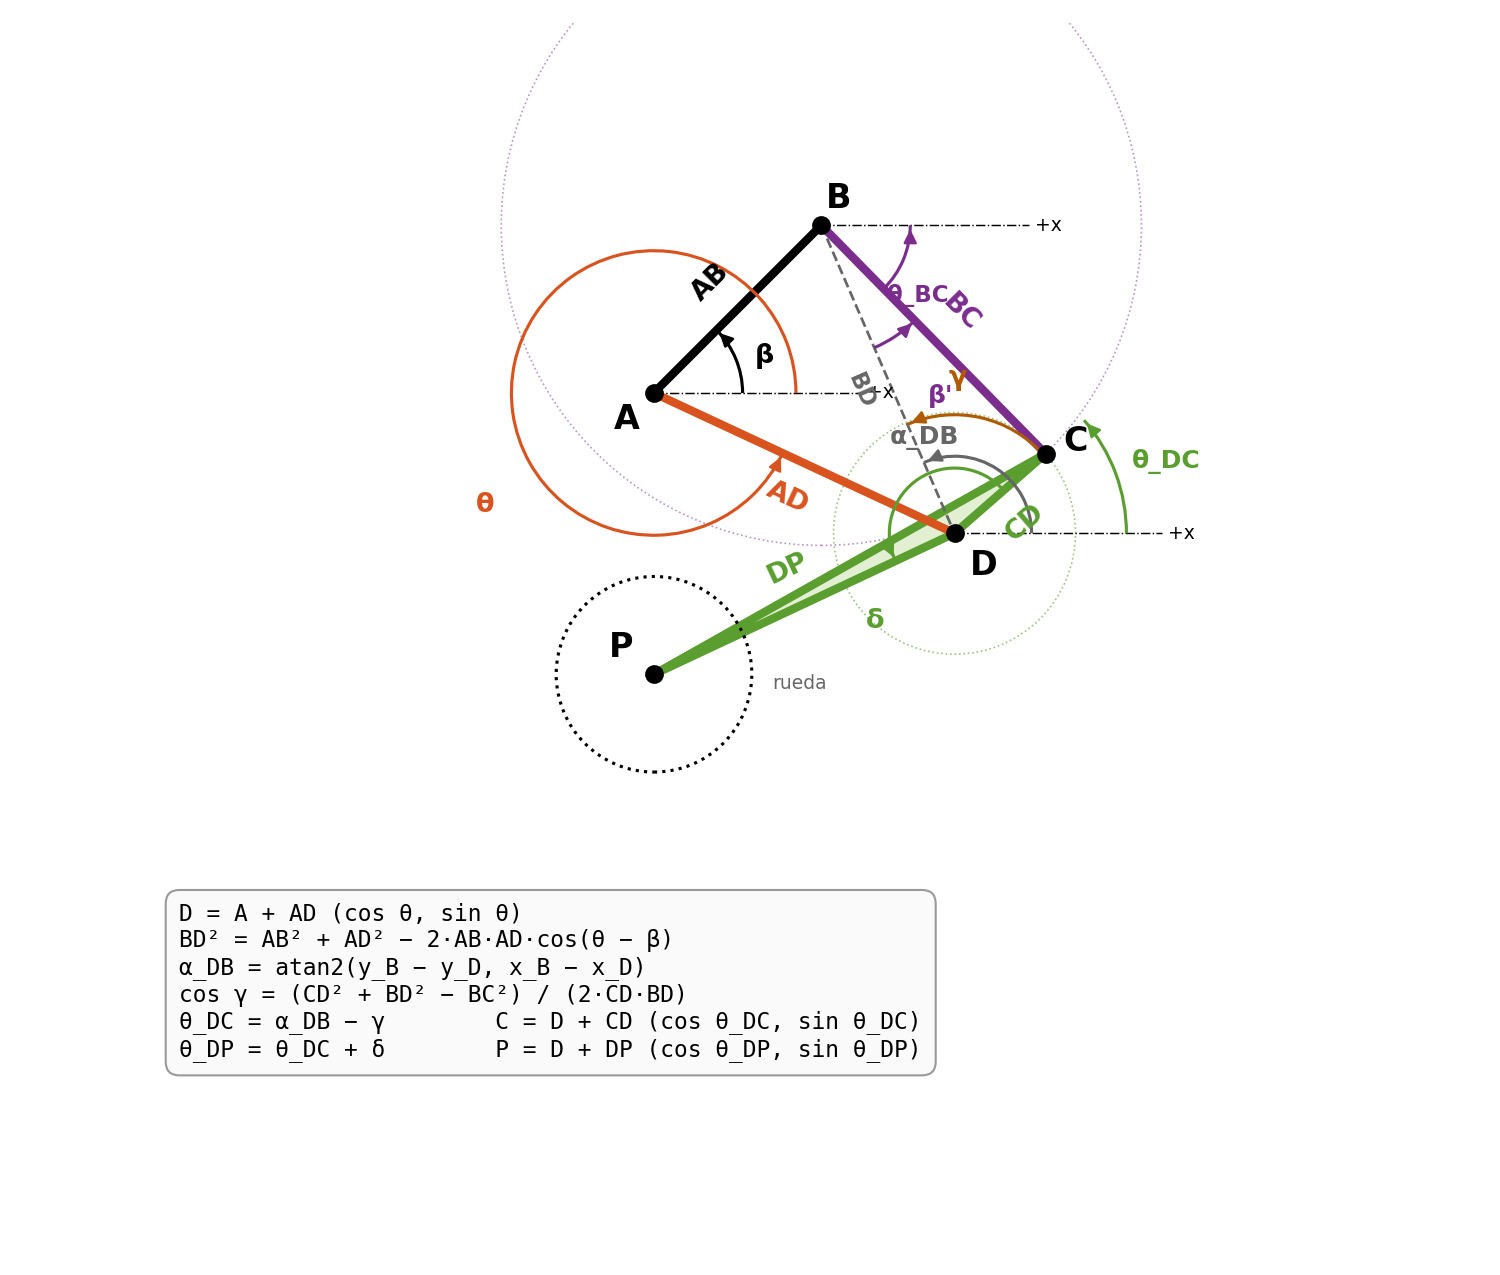
\includegraphics[width=0.95\textwidth]{fig_cinematica_directa.png}
\captionof{figure}{La pata en varias posturas y la trayectoria del eje de la rueda.}
\end{center}

De toda la cinemática, lo que entra en la dinámica es una sola función: $y_P(\theta)$, la
altura del eje de la rueda, y sobre todo su derivada $y_P'(\theta)$. Esa derivada es la
\emph{ventaja mecánica} del mecanismo: cuántos milímetros sube la rueda por cada radián que
gira el servo. Es la que decide cuánto par hace falta.

El desarrollo completo, con todas las derivadas y la verificación numérica, está en el
apéndice \ref{ap:cin}.

% ===========================================================================
\chapter{La pata: dinámica}\label{cap:din}
% ===========================================================================

\begin{idea}
Como el mecanismo tiene un solo grado de libertad, toda su dinámica se reduce a una ecuación
escalar en $\theta$. Lo único que cambia entre el banco de pruebas, el robot parado y el robot
en el aire es \emph{qué está quieto}, y eso entra como un solo vector.
\end{idea}

\section{Una ecuación, tres situaciones}

Por Lagrange, con $\theta$ como coordenada generalizada:

\begin{equation}\label{eq:pata}
I_{eq}(\theta)\,\ddot\theta
\;+\;\tfrac12\,I_{eq}'(\theta)\,\dot\theta^{\,2}
\;+\;V'(\theta)
\;=\;\tau \;-\; b\,\dot\theta \;+\; N\,y_P'(\theta).
\end{equation}

El término $\tfrac12 I_{eq}'\dot\theta^2$ es el de Coriolis y centrífugo: aparece porque la
inercia equivalente \emph{cambia} con la postura. $V'(\theta)$ es el par que hace la gravedad.
$N$ es la normal del piso, que sólo actúa cuando la rueda apoya.

Los tres casos difieren en un solo vector, $u(\theta)$, que es la velocidad de la cabina por
unidad de $\dot\theta$:

\begin{center}
\begin{tabular}{@{}llp{7.0cm}@{}}
\toprule
\textbf{Caso} & $u(\theta)$ & \textbf{Qué representa} \\
\midrule
\texttt{banco} & $0$ & la cabina está amurada y sube y baja la rueda \\
\texttt{parado} & $-c_P$ & la rueda apoya y sube y baja la cabina: \textbf{el robot real de pie} \\
\texttt{aire} & $-2S/m$ & nada está quieto; el centro de masa no se mueve \\
\bottomrule
\end{tabular}
\end{center}

\begin{center}
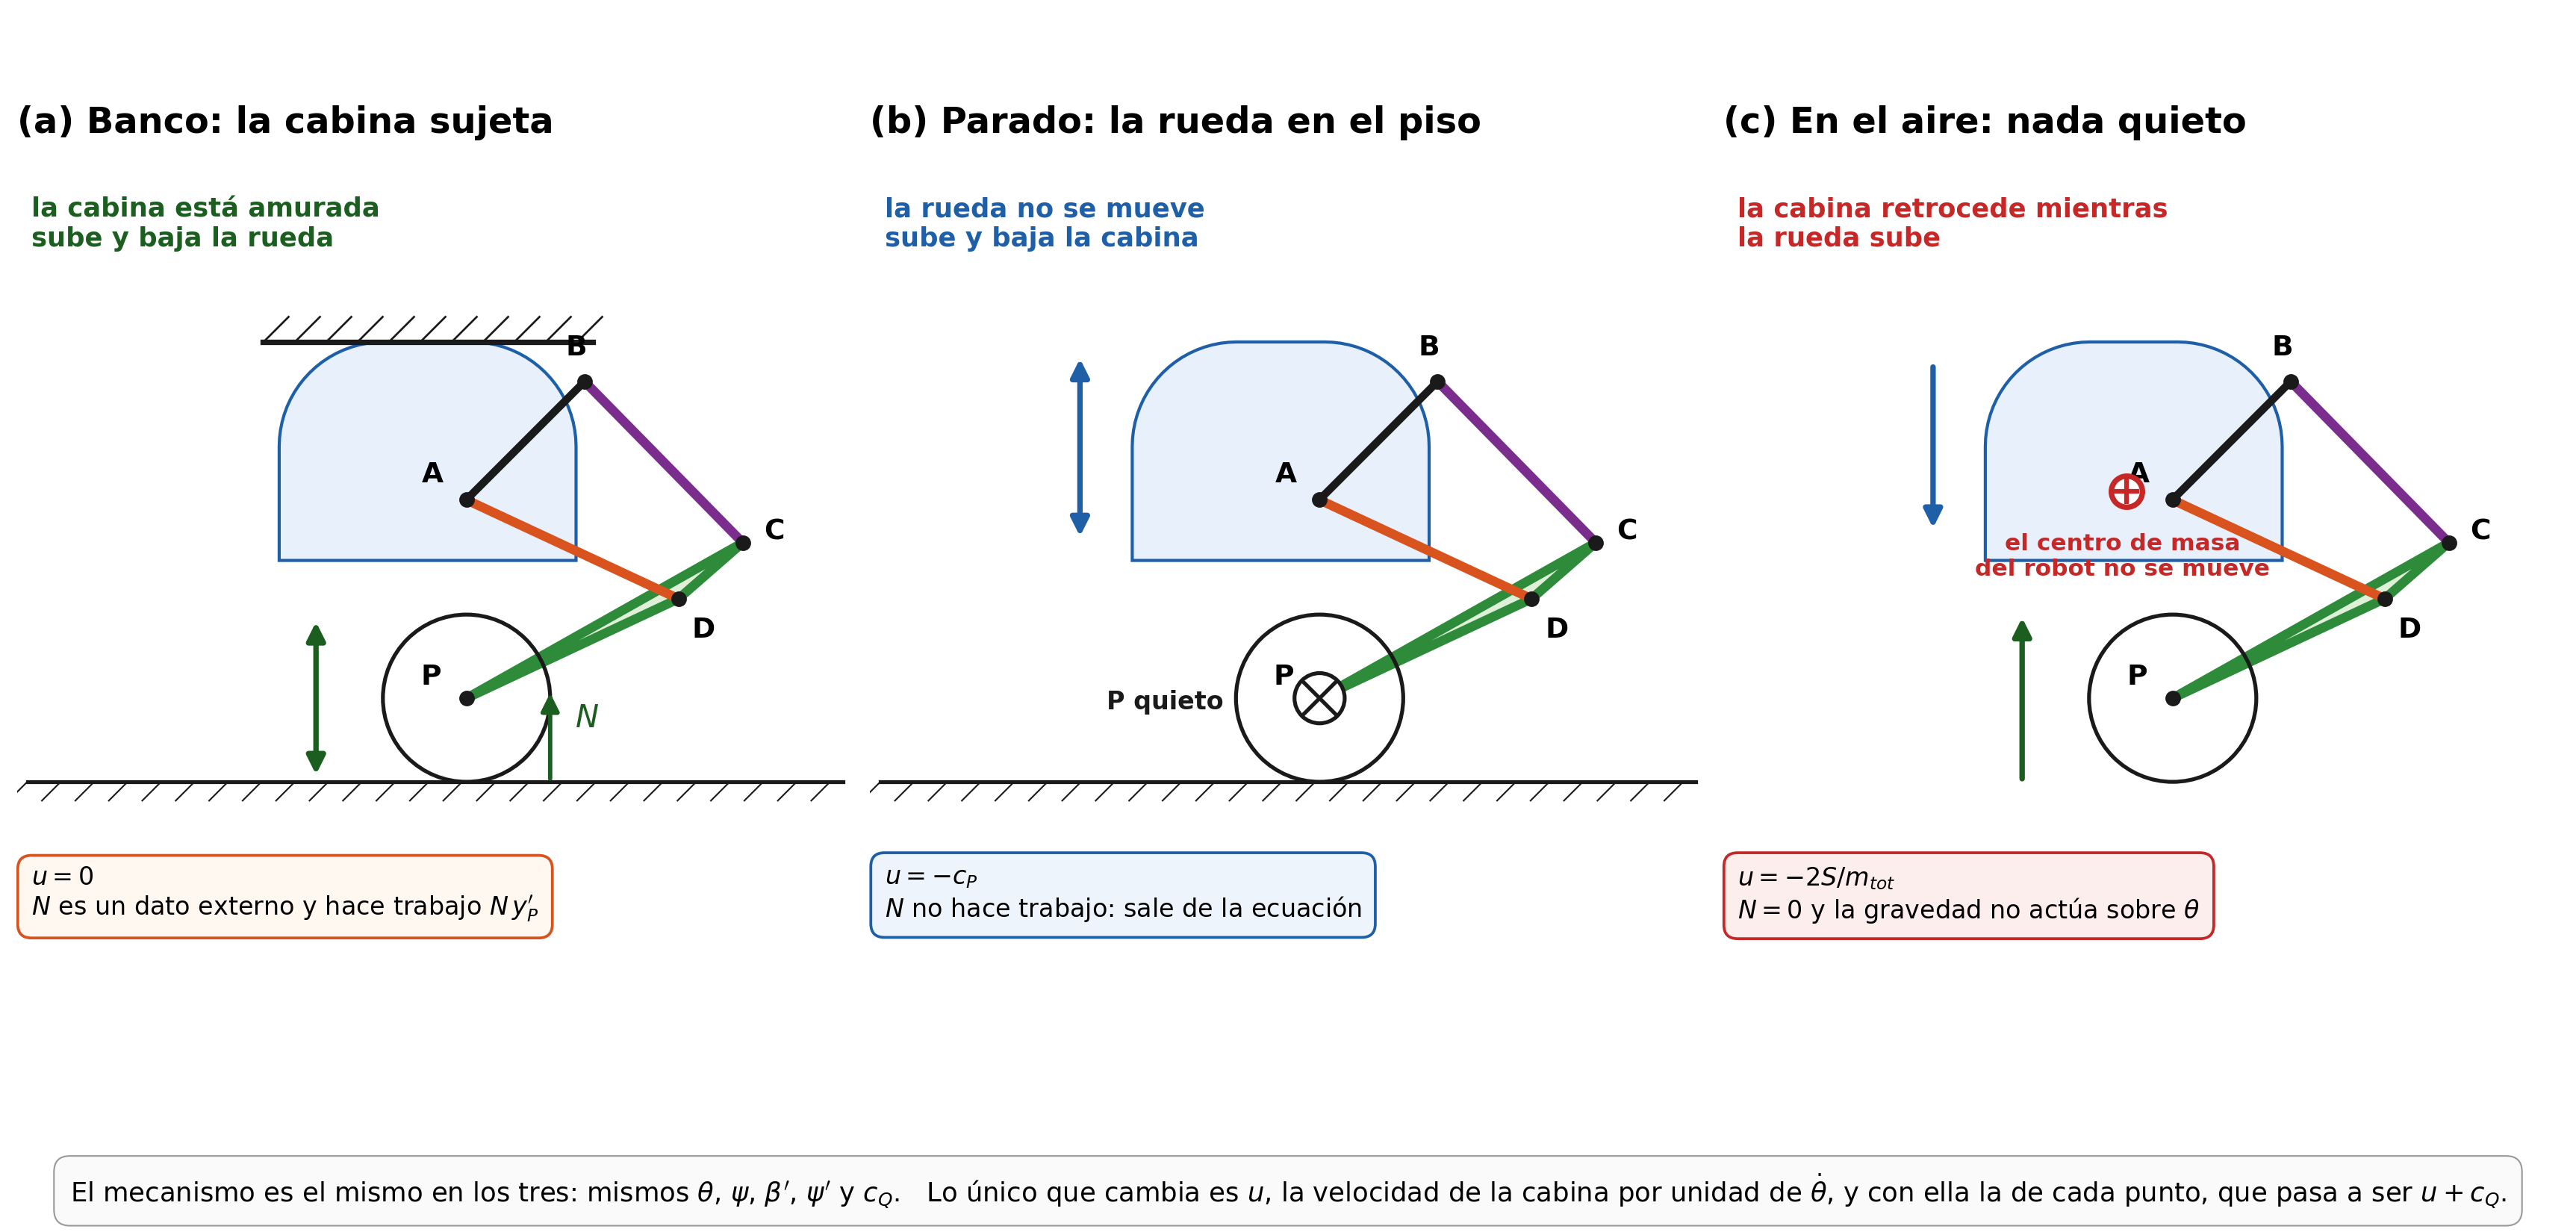
\includegraphics[width=0.95\textwidth]{fig_casos.png}
\captionof{figure}{Los tres casos con el mismo mecanismo. Lo que cambia es qué está quieto.}
\end{center}

\section{Qué sale de ahí}

\begin{center}
\begin{tabular}{@{}lrrr@{}}
\toprule
& $\theta = 10^\circ$ & $\theta = 25^\circ$ & $\theta = 40^\circ$ \\
\midrule
$I_{eq}$ caso \texttt{banco} [g$\cdot$m$^2$] & 8{,}25 & 5{,}40 & 4{,}59 \\
$I_{eq}$ caso \texttt{parado} [g$\cdot$m$^2$] & 19{,}42 & 12{,}30 & 10{,}47 \\
Par estático del servo [kg$\cdot$cm] & \textbf{7{,}98} & 6{,}33 & 5{,}78 \\
\bottomrule
\end{tabular}
\end{center}

Dos lecturas:

\begin{itemize}[leftmargin=1.5em]
\item Parado, el servo ve una inercia \textbf{2{,}3 veces} mayor que en el banco. Tiene
      sentido: en el banco mueve la rueda, parado mueve el robot entero.
\item El peor caso es la pata \textbf{plegada}, con 7{,}98 kg$\cdot$cm por servo. Con el
      DS3240 de 40 kg$\cdot$cm el margen es \textbf{5{,}0}. El servo está holgado.
\end{itemize}

\section{La verificación que vale la pena}

La ecuación \eqref{eq:pata} se obtuvo por Lagrange, que es un método de energías y no muestra
las fuerzas internas. Para comprobarla se resolvió el mismo problema por el camino opuesto:
diagramas de cuerpo libre de las tres barras, nueve ecuaciones de equilibrio con nueve
incógnitas $(A_x, A_y, \tau, B_x, B_y, C_x, C_y, D_x, D_y)$.

\begin{center}
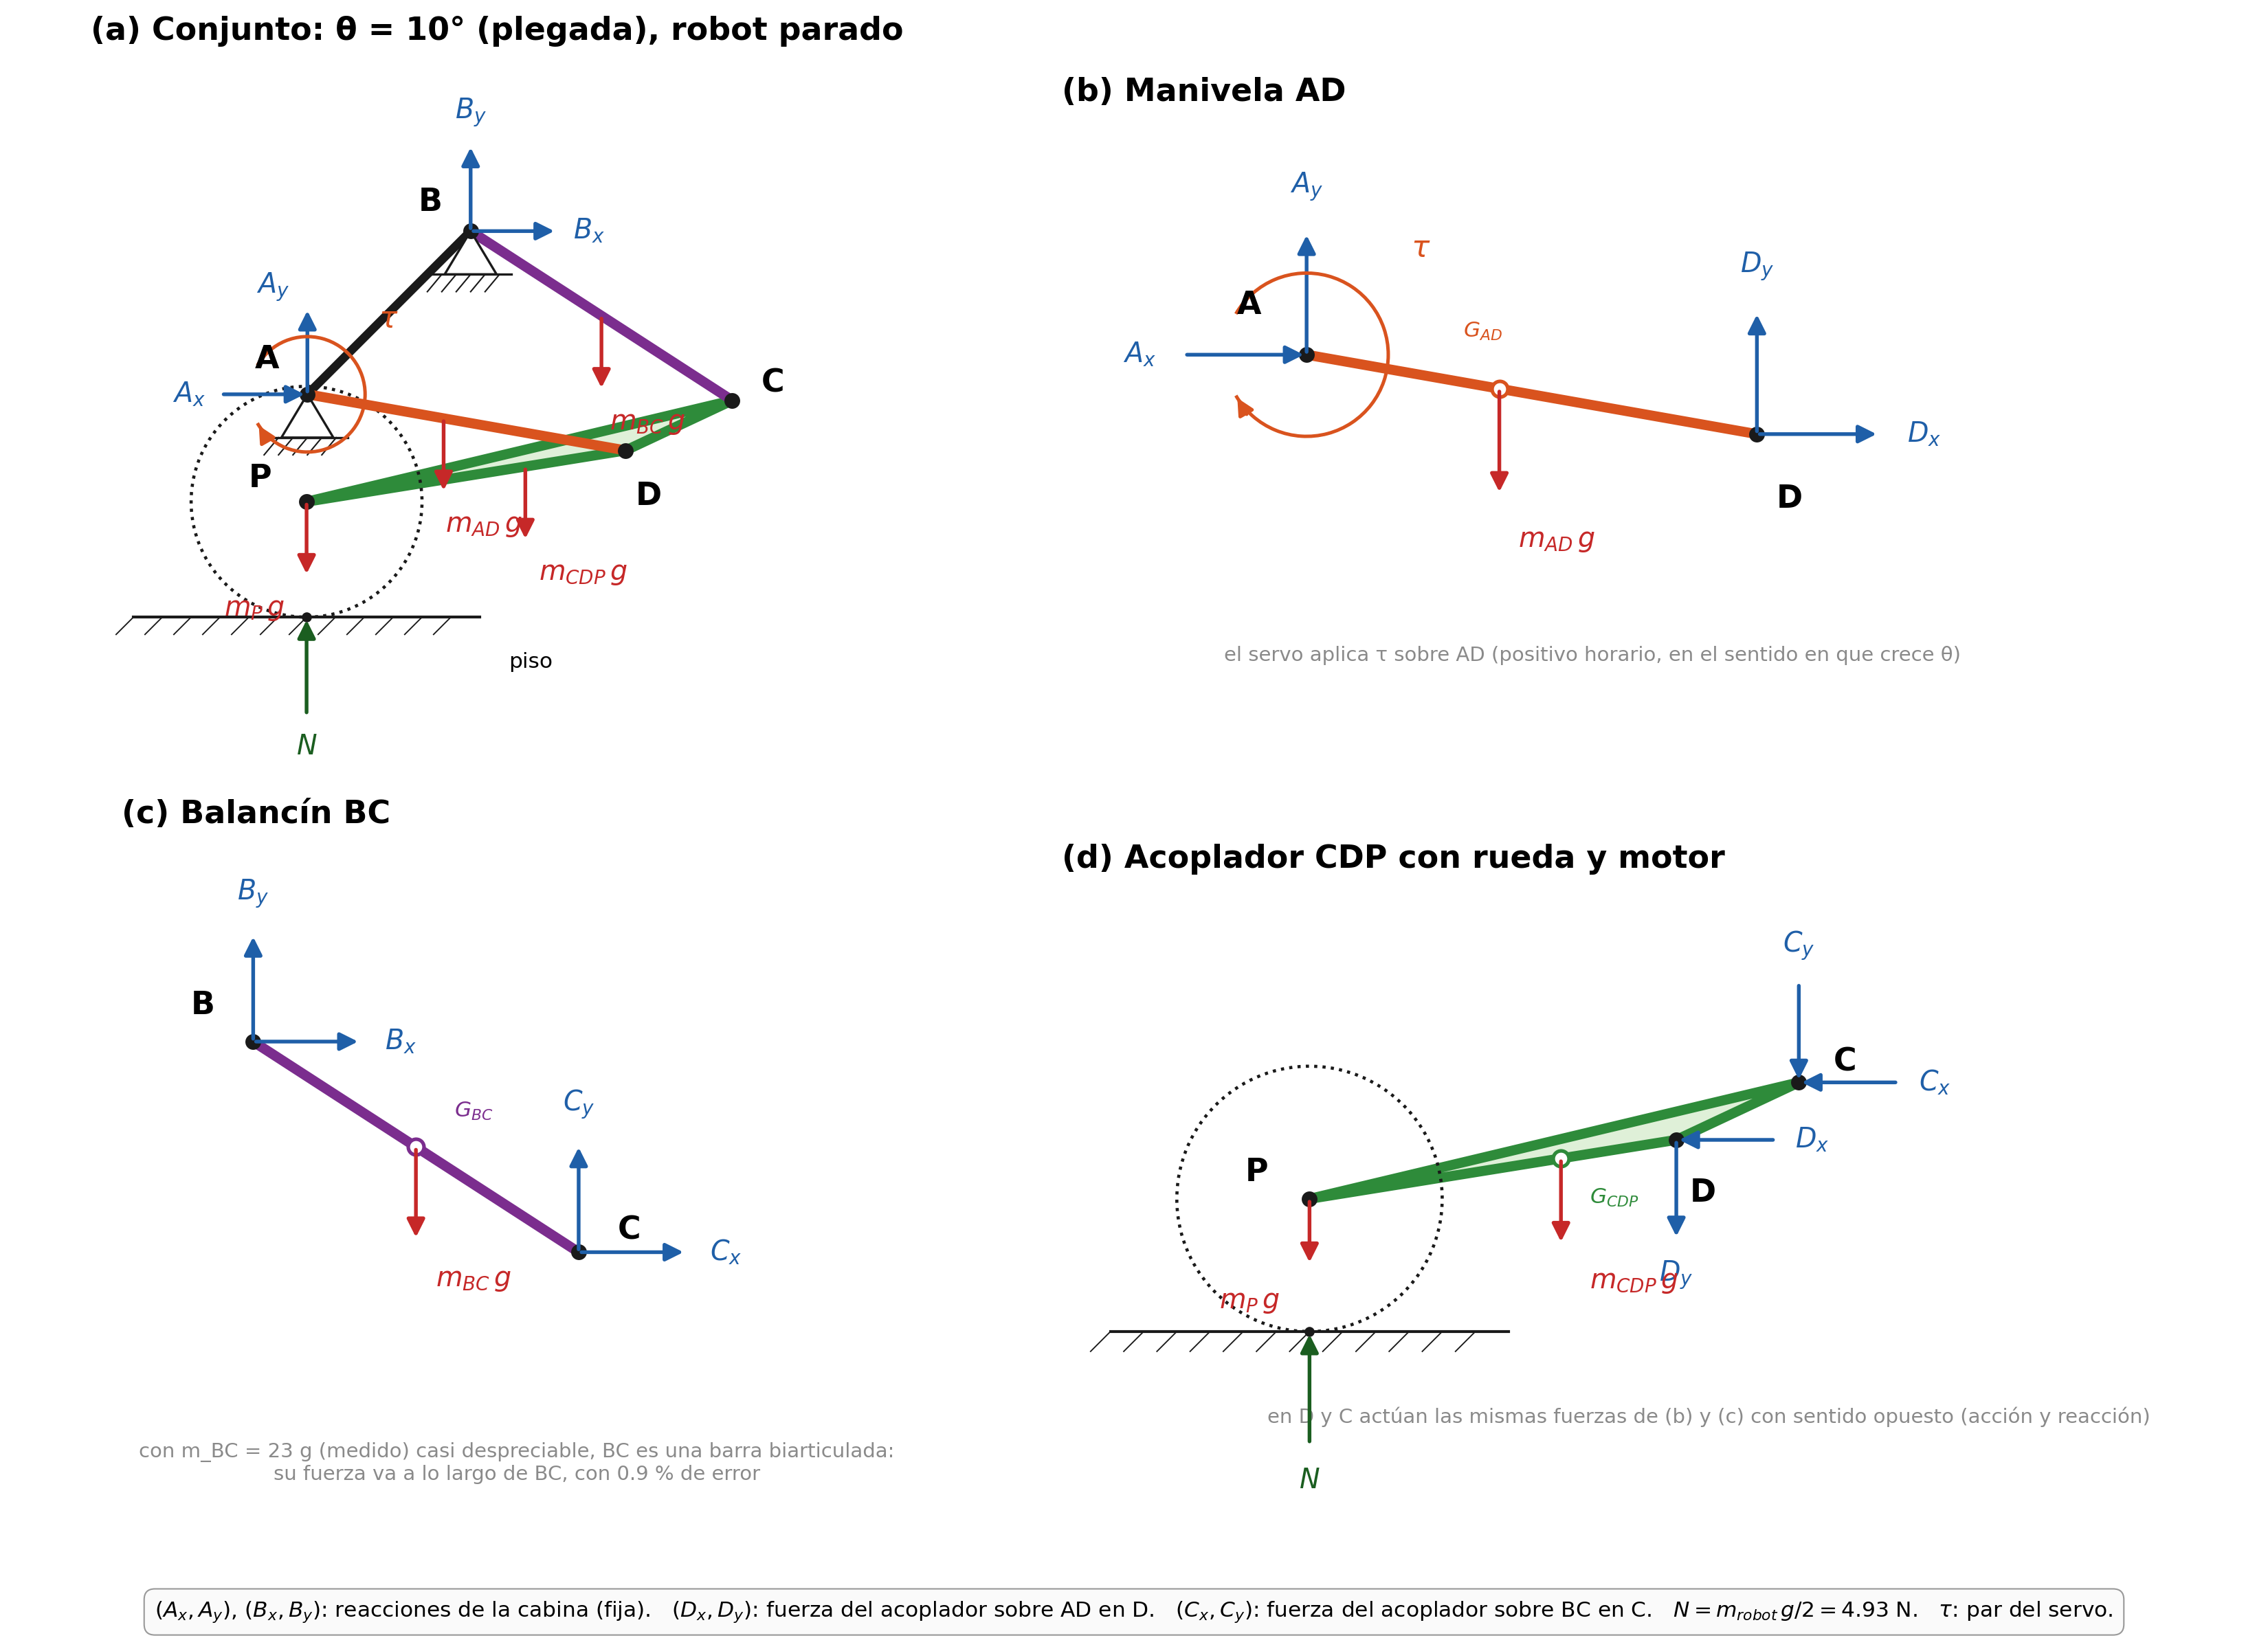
\includegraphics[width=0.95\textwidth]{dcl_pata.png}
\captionof{figure}{Los tres cuerpos de la pata con todas sus fuerzas. Resolver este sistema
da el mismo par que Lagrange hasta el redondeo de máquina.}
\end{center}

Los dos caminos dan el mismo par con una diferencia de $8\times10^{-16}$ N$\cdot$m, que es
precisión de máquina. Son métodos independientes, así que coincidir es evidencia fuerte de
que los dos están bien. El desarrollo está en el apéndice \ref{ap:dcl}.

\section{Aterrizar de un escalón}

\begin{idea}
Cuando el robot cae de un escalón hay \textbf{dos golpes distintos}, y conviene no
confundirlos, porque los absorben cosas distintas.
\end{idea}

\begin{center}
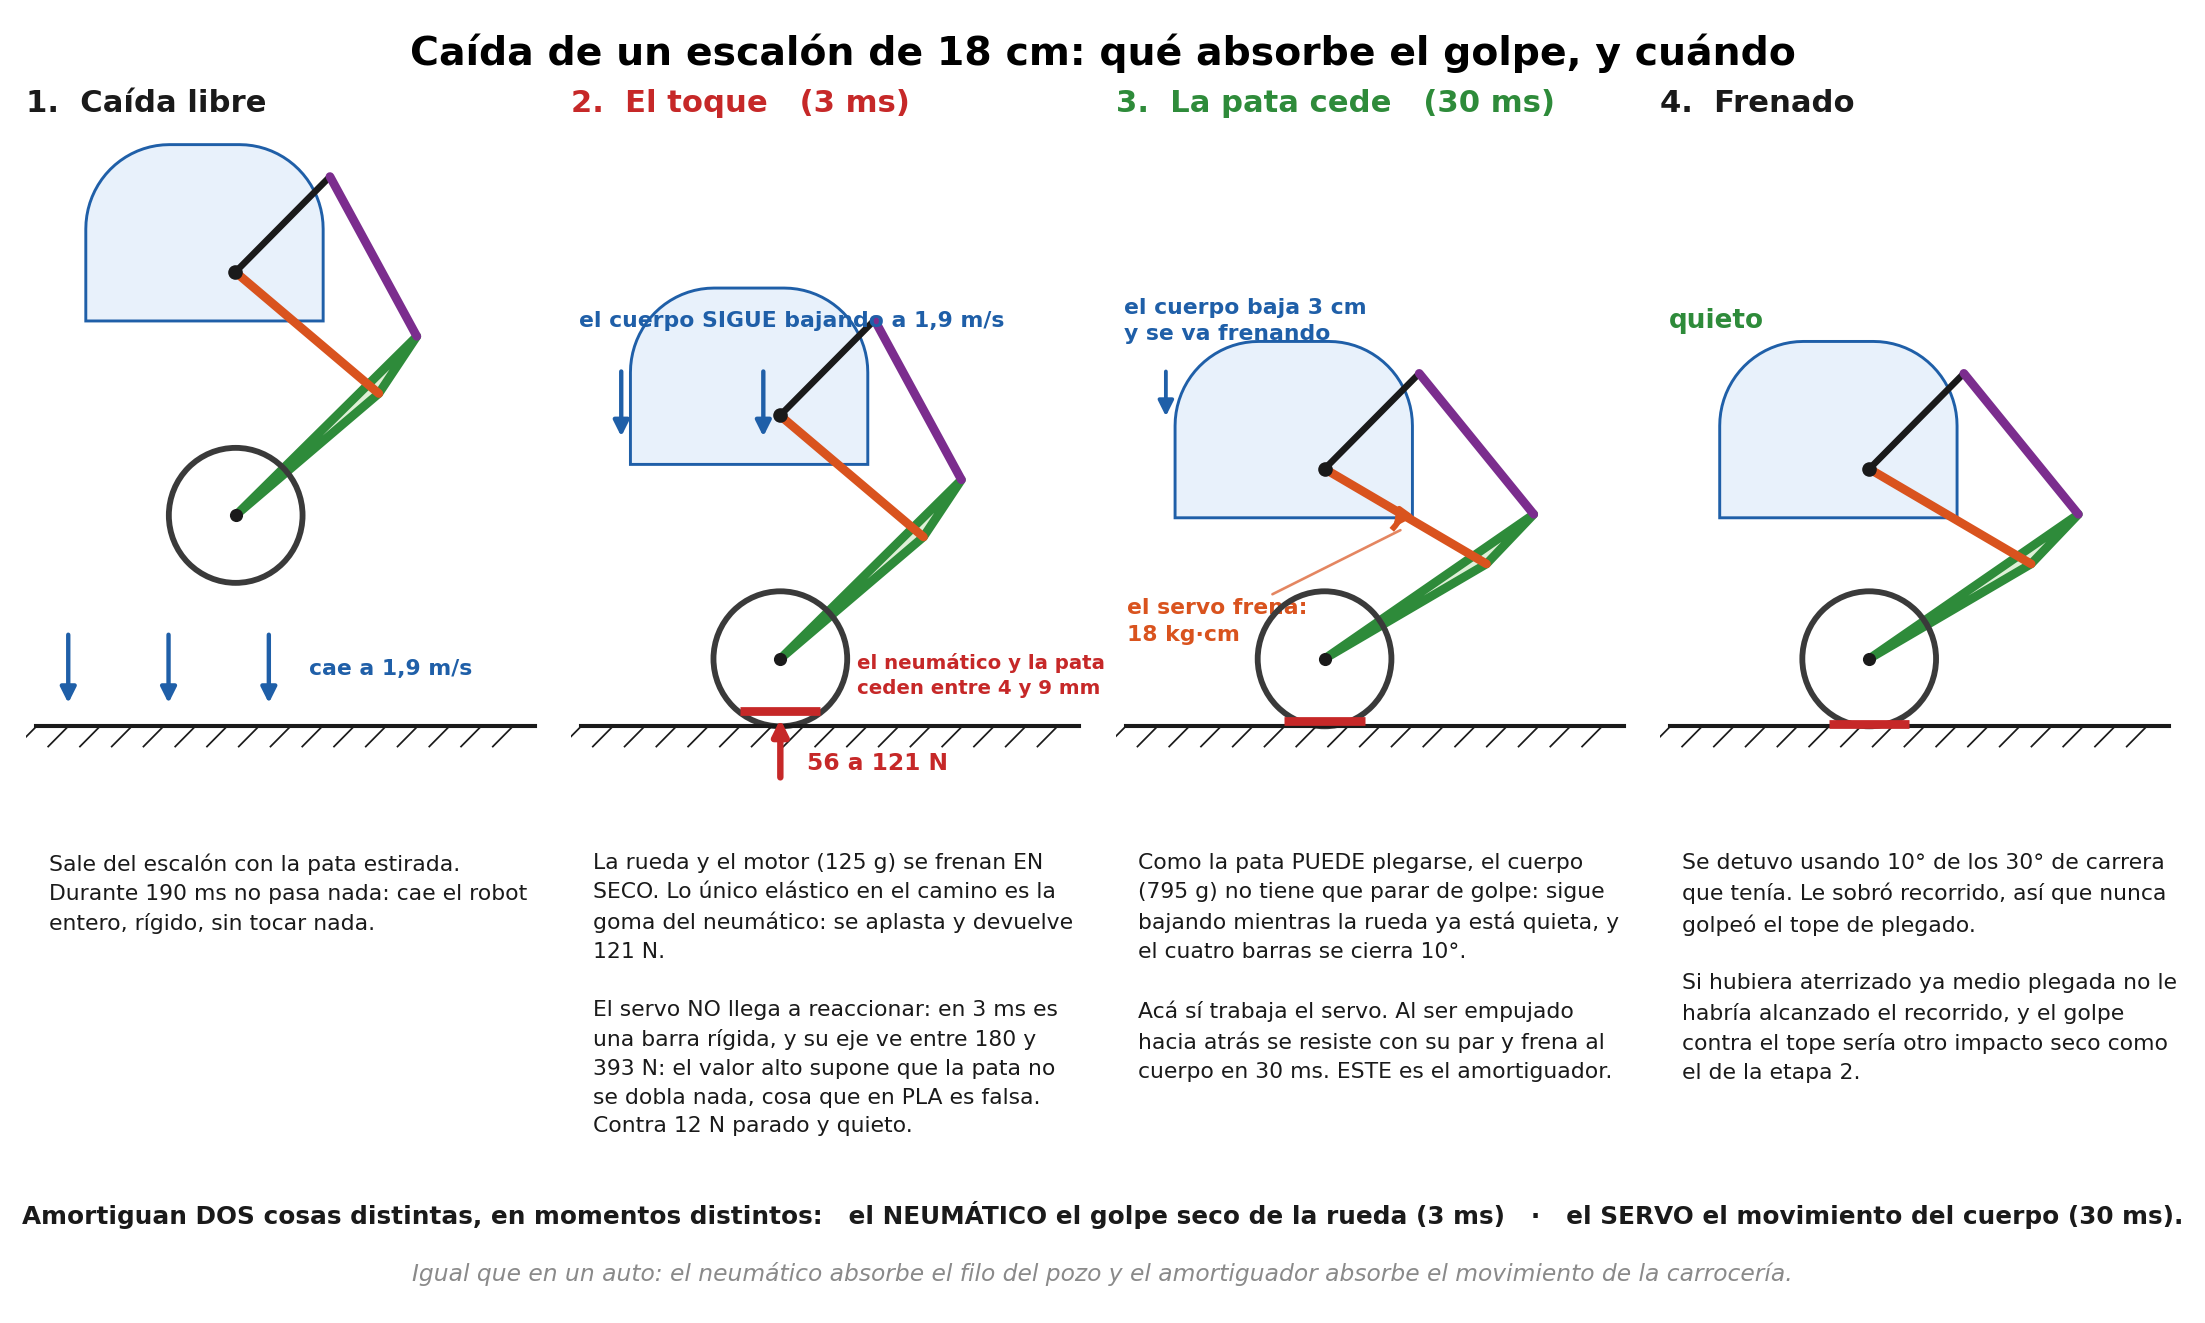
\includegraphics[width=\textwidth]{fig_aterrizaje.png}
\captionof{figure}{La secuencia del aterrizaje desde un escalón de 18 cm.}
\end{center}

\begin{center}
\begin{tabular}{@{}lll@{}}
\toprule
& \textbf{Fase A: el toque} & \textbf{Fase B: el frenado} \\
\midrule
Dura & $\sim$3 ms & 11 a 33 ms \\
Qué se frena & la rueda y el motor, 125 g, en seco & el resto del robot, 795 g \\
Quién lo absorbe & \textbf{sólo el neumático} & el servo plegando la pata \\
El servo & no reacciona: es una barra rígida & trabaja, 8 a 18 kg$\cdot$cm \\
Fuerza en el eje del servo & 128 N (2 cm) a 393 N (18 cm) & 71 N \\
\bottomrule
\end{tabular}
\end{center}

La fase B está cubierta: el servo absorbe 0{,}9 J usando 10 de los 30 grados de carrera.
La que preocupa es la fase A.

\begin{ojo}
En 3 ms el servo no llega a reaccionar: mantiene posición y transmite todo. El pico sale de
$F = \sqrt{2Ek}$, con $E$ la energía de la masa \emph{no suspendida} (rueda más motor) y $k$
la rigidez del neumático. Un neumático tres veces más blando baja el pico un 43\%; uno tres
veces más duro lo sube un 74\%.

La recomendación de diseño que sale de acá: que el pasador $A$ tenga \textbf{rodamiento
propio} tomando la carga radial, y que el servo entregue sólo par. 393 N sobre el estriado de
un servo le arranca los dientes.
\end{ojo}

% ===========================================================================
\chapter{El péndulo invertido: la planta que se controla}\label{cap:pend}
% ===========================================================================

\begin{idea}
Con las patas congeladas, el robot es un péndulo invertido sobre ruedas: dos grados de
libertad, $x$ (avance) y $\varphi$ (inclinación), y una sola entrada, el par de los motores.
Un actuador para dos coordenadas: por eso el problema no es trivial.
\end{idea}

\section{Las coordenadas}

\begin{center}
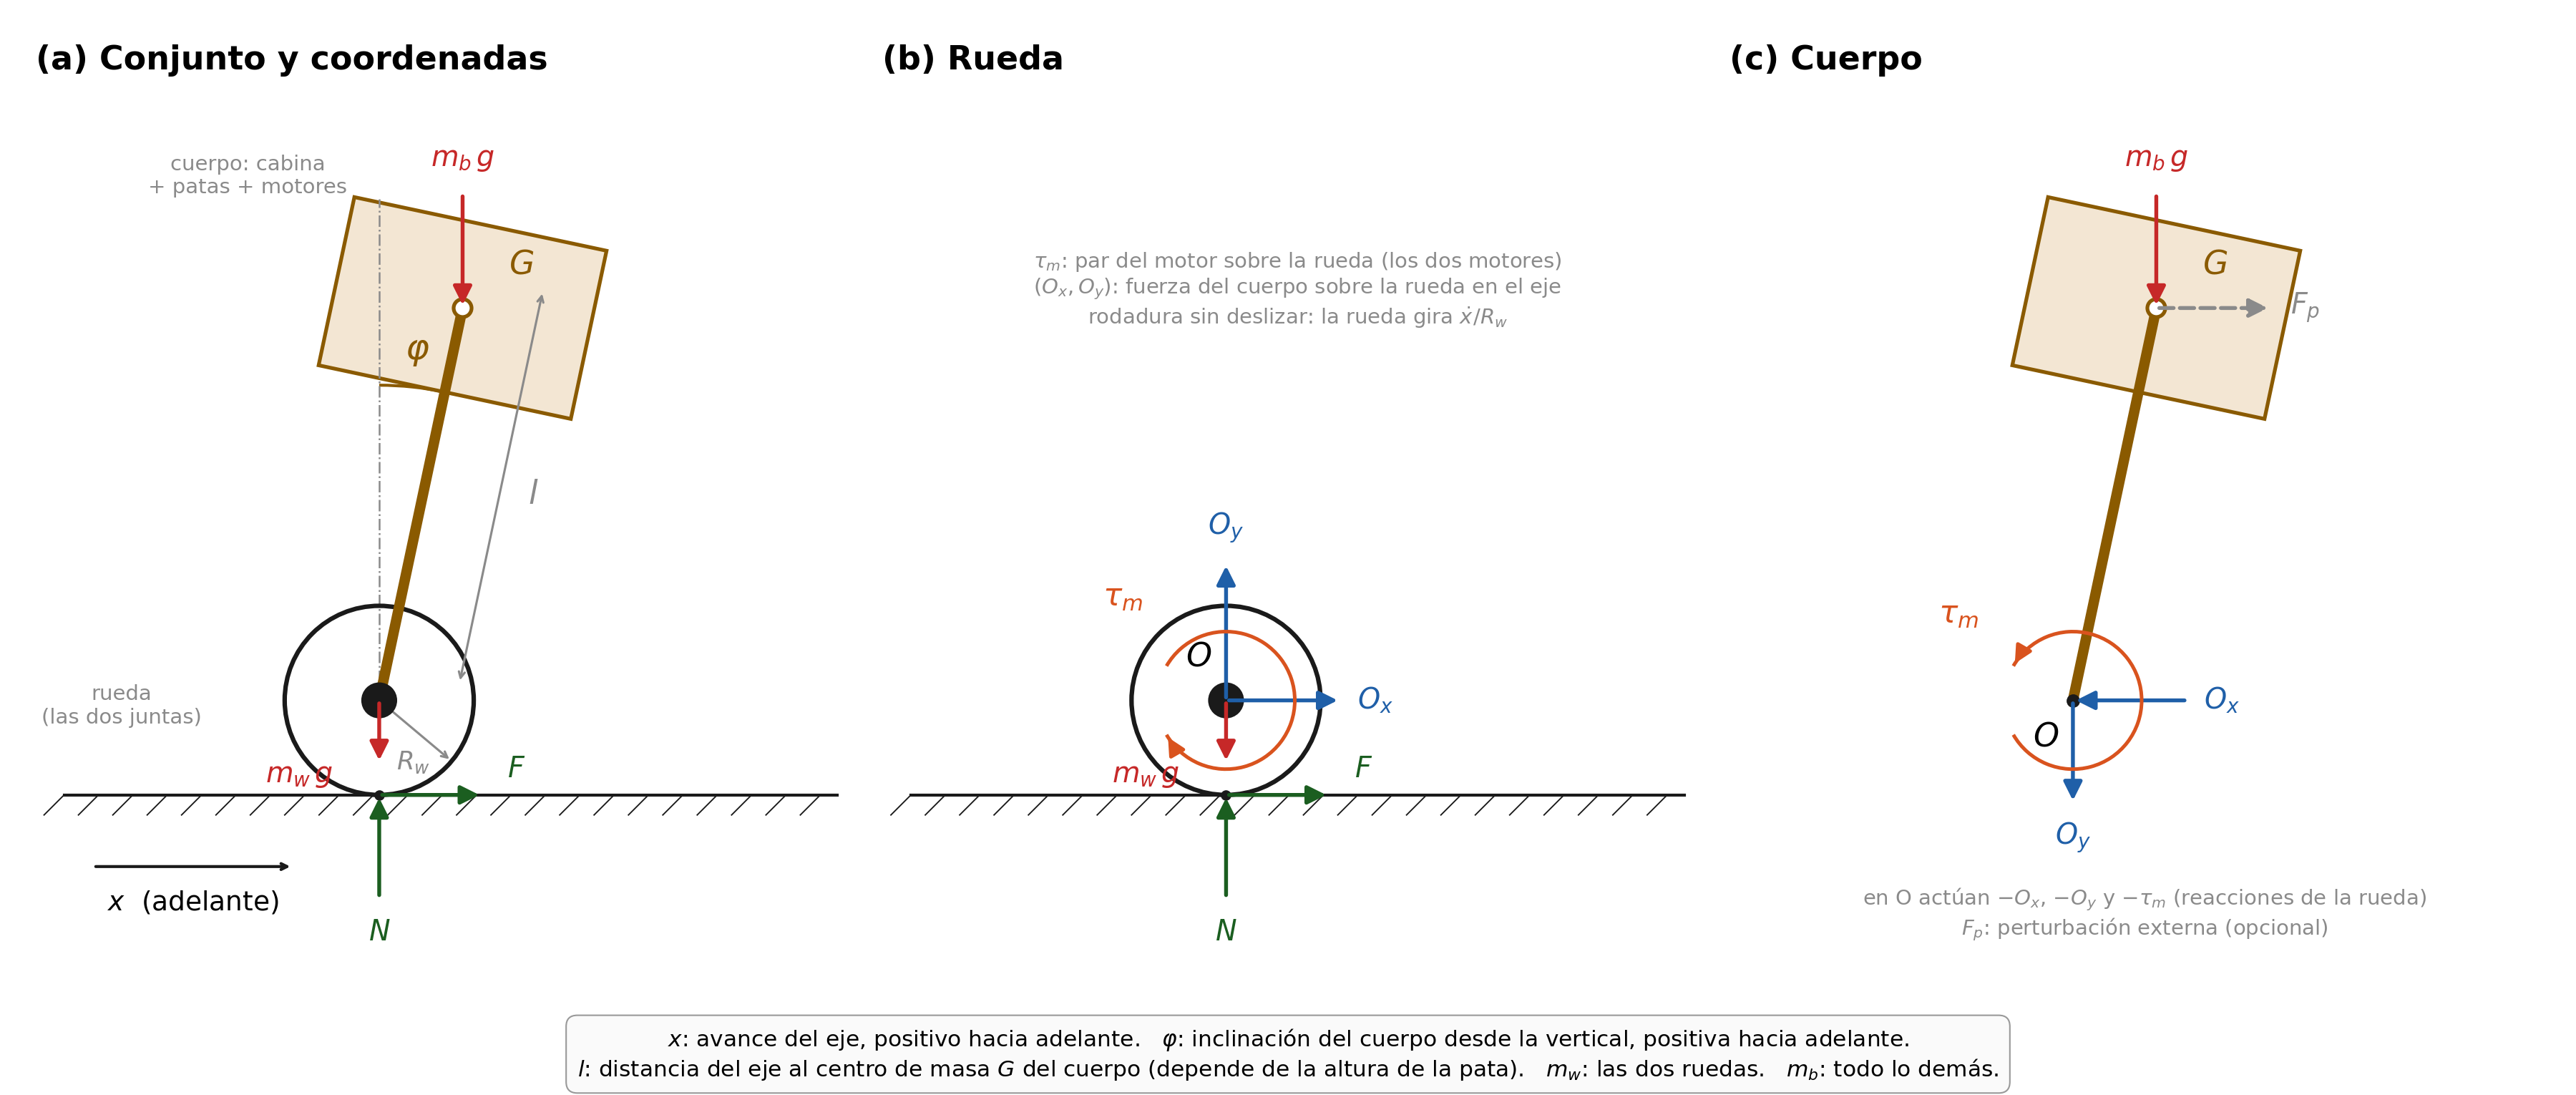
\includegraphics[width=0.78\textwidth]{dcl_segway.png}
\captionof{figure}{Los dos cuerpos: la rueda (las dos juntas) y el cuerpo (cabina, patas y
motores). $x$ es el avance del eje, positivo hacia adelante, y $\varphi$ la inclinación del
cuerpo desde la vertical, positiva hacia adelante.}
\end{center}

La rueda rueda sin deslizar, así que gira $\dot x / R_w$. Los motores aplican $\tau$ sobre la
rueda y, por reacción, $-\tau$ sobre el cuerpo. Ese par de reacción es \emph{la única forma}
que tiene el robot de inclinarse a voluntad.

\begin{ojo}
$\varphi$ \textbf{no} es el ángulo del chasis. Se mide desde la dirección del centro de masa,
que no coincide con la vertical del chasis: hay entre medio un ángulo $\delta_G$ que vale
$3{,}58^\circ$ en la postura media. La IMU mide el chasis, así que el firmware tiene que
sumarle $\delta_G$. El capítulo \ref{cap:patasmov} muestra qué pasa si no lo hace.
\end{ojo}

\section{Las ecuaciones}

Con $q = [x;\ \varphi]$, las ecuaciones de Lagrange quedan en forma matricial:

\begin{equation}\label{eq:planta}
\boxed{\;M(\varphi)\,\ddot q \;=\; H\,\tau \;-\; D\,\dot q \;+\; \sin\varphi
\begin{bmatrix} -h\,\dot\varphi^{\,2} \\ k \end{bmatrix}\;}
\end{equation}

con
\begin{equation}
M(\varphi) = \begin{bmatrix}
a & -h\cos\varphi + e \\[2pt]
-h\cos\varphi + e & j
\end{bmatrix},
\qquad
H = \begin{bmatrix} -1/R_w \\ -1 \end{bmatrix},
\qquad
D = \begin{bmatrix} b_x & 0 \\ 0 & b_\varphi \end{bmatrix}.
\end{equation}

Cada coeficiente tiene un significado físico directo:

\begin{center}
\begin{tabular}{@{}llr@{}}
\toprule
\textbf{Coef.} & \textbf{Qué es} & \textbf{Valor a $25^\circ$} \\
\midrule
$a$ & masa que hay que acelerar para avanzar, incluida la inercia de ruedas y rotores & 1{,}2499 kg \\
$h$ & acoplamiento entre avance e inclinación: $m_b\,\ell$ & 0{,}0702 kg$\cdot$m \\
$j$ & inercia del cuerpo alrededor del eje de la rueda & 0{,}010018 kg$\cdot$m$^2$ \\
$k$ & par que hace la gravedad por radián: $m_b\,g\,\ell$ & 0{,}6891 N$\cdot$m \\
$e$ & acoplamiento del rotor, constante (ver abajo) & 0{,}011400 \\
\bottomrule
\end{tabular}
\end{center}

\begin{ojo}
El término $e$ es sutil y costó entenderlo. La velocidad del rotor del motor es
$\dot\alpha_m = -n\,\dot x/R_w + (1-n)\,\dot\varphi$, con $n$ la reducción. Es
\emph{lineal con coeficientes fijos}: no depende de $\varphi$. Por eso su contribución a
$M_{12}$ es una constante y \textbf{no} puede meterse dentro de $h$, que sí va multiplicado
por $\cos\varphi$. Con $e = 0$ se recupera el modelo clásico sin rotor.
\end{ojo}

\section{Linealizar}

Alrededor de $\varphi = 0$, $\dot\varphi = 0$, con $\cos\varphi \to 1$ y $\sin\varphi \to
\varphi$, el término cuadrático desaparece y queda un sistema lineal
$\dot z = A z + B\,U$ con $z = [x;\ v;\ \varphi;\ \omega]$:

\begin{equation}
A = \begin{bmatrix}
0 & 1 & 0 & 0\\
0 & -16{,}522 & 4{,}476 & -0{,}667\\
0 & 0 & 0 & 1\\
0 & -145{,}352 & 95{,}074 & -5{,}952
\end{bmatrix},
\qquad
B = \begin{bmatrix} 0 \\ -1{,}805 \\ 0 \\ -15{,}880 \end{bmatrix}.
\end{equation}

\section{Qué dicen los polos y los ceros}

\begin{center}
\begin{tabular}{@{}lr p{7.2cm}@{}}
\toprule
\textbf{Qué} & \textbf{Valor} & \textbf{Qué significa} \\
\midrule
Polo inestable & $+7{,}345$ s$^{-1}$ & la inclinación se duplica cada \textbf{94 ms}: ése
es el tiempo que tiene el control para reaccionar \\
Polo rápido & $-24{,}76$ s$^{-1}$ & la fricción eléctrica del motor \\
Polo & $-5{,}06$ s$^{-1}$ & \\
Polo en el origen & $0$ & la posición: nada se opone a que el robot se vaya caminando \\
Cero de $U \to x$ & $+7{,}423$ s$^{-1}$ & \textbf{fase no mínima} \\
Rango de controlabilidad & 4 de 4 & el sistema es controlable: un solo motor alcanza \\
\bottomrule
\end{tabular}
\end{center}

\begin{idea}
El cero en el semiplano derecho es la explicación formal de algo que se ve en cualquier
Segway: \textbf{para ir hacia adelante, primero hay que ir hacia atrás}. El robot retrocede
unos milímetros para inclinarse, y recién entonces avanza. No es un defecto del controlador,
es una propiedad de la planta, y \emph{ningún} control la puede eliminar.
\end{idea}

En la simulación, ese retroceso es de \textbf{13{,}9 mm} antes de avanzar 30 cm.

% ===========================================================================
\chapter{El motor y el límite de tracción}\label{cap:motor}
% ===========================================================================

\begin{idea}
El motor convierte tensión en par, pero no instantáneamente ni gratis: tiene resistencia,
fuerza contraelectromotriz y un rotor que hay que acelerar. Y el par que entrega no se
convierte entero en fuerza contra el piso.
\end{idea}

\section{El modelo del motor}

Con la inductancia despreciada (su constante de tiempo es microsegundos, contra los 94 ms del
péndulo), el motor de corriente continua da:

\begin{equation}
\tau = \beta_V\,U - b_m\,\omega_{rel},
\qquad
\beta_V = \frac{n_{mot}\,\eta\,n_g\,K_t}{R_m},
\qquad
b_m = \frac{n_{mot}\,\eta\,n_g^2\,K_t K_e}{R_m}.
\end{equation}

\begin{center}
\begin{tabular}{@{}llr@{}}
\toprule
\textbf{Parámetro} & \textbf{De dónde sale} & \textbf{Valor} \\
\midrule
$n_g$, reducción & publicación & 20 \\
$K_t = K_e$ & de la velocidad en vacío, corregida por $R_m i_0$ & 0{,}01812 \\
$R_m$ & \textcolor{naranjap}{deducida} de la corriente de vacío & 10{,}28 $\Omega$ \\
$\eta$, rendimiento del reductor & \textcolor{rojop}{supuesto} & 0{,}75 \\
$\beta_V$ & calculado & 0{,}05287 N$\cdot$m/V \\
$b_m$ & calculado & 0{,}019157 N$\cdot$m$\cdot$s/rad \\
$V_{bat}$ & tres celdas & 11{,}1 V \\
\midrule
Par de bloqueo (los dos motores) & calculado & \textbf{0{,}587 N$\cdot$m} \\
Velocidad máxima & calculada & \textbf{1{,}23 m/s} \\
\bottomrule
\end{tabular}
\end{center}

\begin{ojo}
La ficha comercial del GA25-370 \textbf{se contradice sola}: su punto de carga implica un
rendimiento de reductor del 18\% y su punto de bloqueo, del 146\%, que es físicamente
imposible. La columna eléctrica, en cambio, es coherente consigo misma. Por eso el modelo
\emph{calcula} el par (3{,}1 kg$\cdot$cm por motor) en lugar de \emph{leerlo} (5{,}6
declarados). Hay que medirlo: ensayo M-2.
\end{ojo}

\section{La trampa del límite de tracción}

\begin{ojo}
\textbf{$\tau/R_w$ no es la fuerza en el contacto.} Es el error que ya cometimos una vez, y
cambió una conclusión publicada.

Parte del par del motor no va al piso: va a acelerar la inercia reflejada del rotor, que con
una reducción de 1:20 equivale a un tercio de kilo sobre un robot de un kilo. La fuerza real es
\[
F = c_1\,\tau, \qquad c_1 = \begin{bmatrix} m_{tot} & -h\end{bmatrix} M_0^{-1} H
= -10{,}31 \ \mathrm{N/(N\cdot m)},
\]
contra los $1/R_w = 25{,}0$ que daría la cuenta ingenua. O sea casi \textbf{dos veces y media menos}.
\end{ojo}

Con los números de hoy:

\begin{center}
\begin{tabular}{@{}lr@{}}
\toprule
Fuerza que el motor pone en el piso, a fondo & 6{,}05 N \\
Fricción disponible ($\mu = 0{,}7$ supuesto) & 6{,}32 N \\
\midrule
\textbf{Uso del agarre} & \textbf{96\%} \\
\bottomrule
\end{tabular}
\end{center}

O sea: el motor queda justo por debajo del agarre, pero con un margen de apenas 4\%, y ese
veredicto descansa en $\mu = 0{,}7$, que está supuesto. El capítulo \ref{cap:falta} explica
cómo medirlo y por qué, a pesar de todo, no es grave.

\begin{center}
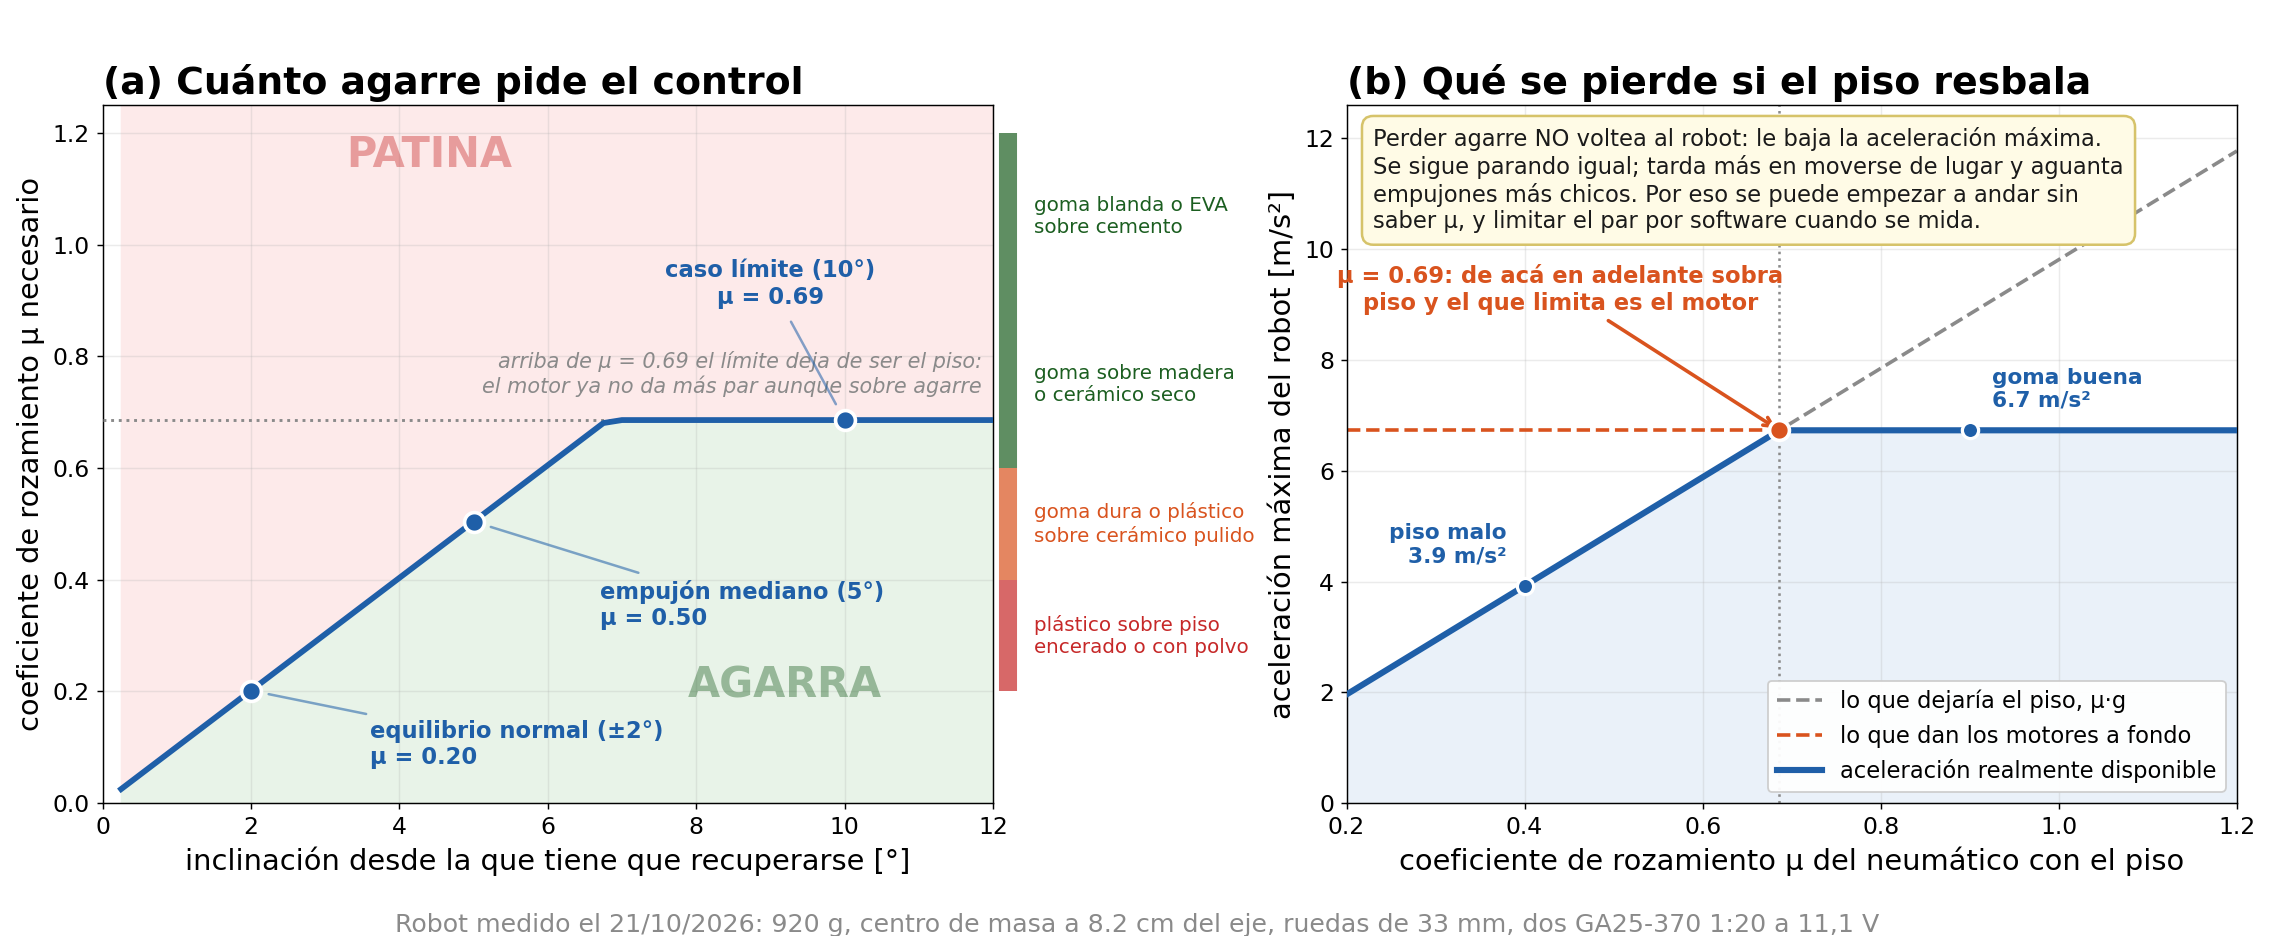
\includegraphics[width=\textwidth]{fig_traccion.png}
\captionof{figure}{Cuánto agarre pide el control en cada maniobra, y qué se pierde si el piso
resbala.}
\end{center}

% ===========================================================================
\chapter{El controlador: por qué LQR}\label{cap:lqr}
% ===========================================================================

\begin{idea}
Hay que estabilizar un sistema inestable con dos coordenadas y un solo actuador. El LQR no es
el único método que funciona, pero es el único que escala a ese problema sin que haya que
adivinar nada.
\end{idea}

\section{La justificación que se puede defender}

\begin{enumerate}[leftmargin=1.6em]
\item \textbf{Un PID no alcanza.} Un PID controla una salida. Acá hay dos coordenadas que
      importan, $x$ y $\varphi$, y un solo actuador. Realimentando sólo el ángulo el robot
      se equilibra pero \textbf{la posición queda siempre inestable}: se va caminando. Está
      verificado en el capítulo \ref{cap:simulink}.
\item \textbf{Con realimentación de estado hay que elegir cuatro ganancias a la vez.} Ubicar
      polos funciona, pero elegir cuatro polos de un sistema de cuarto orden a mano es
      adivinar. El LQR convierte esa elección en algo que se puede justificar: cuánto
      \emph{molesta} cada error y cuánta tensión se está dispuesto a gastar.
\item \textbf{La regla de Bryson le da sentido físico a los pesos.} Se pesa cada estado por
      el inverso del cuadrado de su valor máximo tolerable. Acá: 10 cm de error de posición,
      30 cm/s, $8^\circ$ de inclinación, 1 rad/s.
\item \textbf{El LQR regala márgenes.} La desigualdad de Kalman garantiza margen de fase
      $\geq 60^\circ$ y margen de ganancia infinito hacia arriba, \emph{por construcción}.
      Acá el margen de fase medido es $94^\circ$.
\end{enumerate}

\begin{ojo}
Para un sistema de una sola entrada, LQR y ubicación de polos dan \emph{exactamente} el mismo
controlador si se ubican los polos donde el LQR los puso (verificado a $10^{-12}$). Así que el
argumento a favor del LQR no puede ser sobre el resultado: es sobre el \textbf{método}. El LQR
te dice dónde poner los polos; ubicación de polos te pide que ya lo sepas.
\end{ojo}

\section{Los pesos, y una corrección que importó}

\begin{equation}
Q = \mathrm{diag}\!\left(\frac{1}{0{,}10^2},\ \frac{1}{0{,}30^2},\
\frac{1}{(8^\circ)^2},\ \frac{1}{1^2}\right)
= \mathrm{diag}(100{,}0,\ 11{,}1,\ 51{,}3,\ 1{,}0),
\qquad
R = \frac{f_R}{V_{bat}^2}.
\end{equation}

\begin{ojo}
Con la regla de Bryson pura ($f_R = 1$) el diseño es impecable en el papel y
\textbf{no sobrevive a la implementación}. Pone un polo en $-189$ s$^{-1}$ que no tiene nada
que ver con la física del robot (el más rápido de la planta es $-27$): es puro costo de
muestreo. Con un período de 5 ms, un paso de retardo y el filtro de 20 Hz que la cuantización
del encoder obliga, el lazo queda \textbf{inestable}, con radio espectral 1{,}178.

Con $f_R = 4$: radio espectral 0{,}985, el margen de muestreo pasa de 1{,}2$\times$ a
2{,}6$\times$ y el ruido del encoder cae de 4{,}4 a 2{,}6 V. Cuesta un 8\% de tiempo de
respuesta. \textbf{Es una de las decisiones más importantes del proyecto}, y no aparece en
ningún libro: aparece al simular la implementación real.
\end{ojo}

\section{El controlador que quedó}

\begin{equation}
U = -K\,(z - z_{ref}), \qquad
K = \begin{bmatrix} 55{,}50 & 52{,}87 & -90{,}72 & -11{,}51 \end{bmatrix}
\end{equation}

en voltios por (m, m/s, rad, rad/s).

\begin{center}
\begin{tabular}{@{}lr@{}}
\toprule
Polos a lazo cerrado & $-97{,}54$;\ $-7{,}17$;\ $-2{,}54 \pm 1{,}24i$ \\
Tiempo de asentamiento & 1{,}57 s \\
Margen de fase & $94{,}5^\circ$ a 83{,}9 rad/s \\
Pico de sensibilidad $\|S\|_\infty$ & 1{,}00 \\
\bottomrule
\end{tabular}
\end{center}

Un pico de sensibilidad de 1{,}00 es lo mejor que se puede pedir: significa que el lazo no
amplifica ninguna perturbación en ninguna frecuencia.

% ===========================================================================
\chapter{Simulink: cómo correrlo}\label{cap:simulink}
% ===========================================================================

\begin{idea}
Hay un solo archivo que abrir. Construye el modelo si falta, lo simula, lo compara contra una
integración independiente en MATLAB, y deja figura y resumen en \texttt{resultados/}.
\end{idea}

\section{El archivo que se abre}

\begin{center}
\texttt{simulacion/pendulo\_invertido/INICIAR\_PENDULO\_SIMULINK.m}
\end{center}

Se abre y se pulsa \textbf{Run}. No hace falta nada más: el script agrega las rutas, lee los
parámetros, diseña el LQR, construye el \texttt{.slx} si no existe, simula y verifica.

\section{Las variables en el workspace}

El archivo es un \emph{script}, no una función. Eso es a propósito: todo lo que calcula queda
en el \textbf{workspace base}, que es justamente de donde Simulink lee sus parámetros. Al
terminar quedan disponibles:

\begin{center}
\small
\begin{tabular}{@{}llp{6.4cm}@{}}
\toprule
\textbf{Grupo} & \textbf{Variables} & \textbf{Qué son} \\
\midrule
Parámetros físicos & \texttt{fisicos} & la estructura cruda, en unidades de ingeniería \\
Planta & \texttt{p} & todo el péndulo en SI \\
& \texttt{a h j k e\_acople r} & los coeficientes de la ecuación \eqref{eq:planta} \\
& \texttt{b\_eje b\_x b\_phi} & fricciones \\
Motor & \texttt{motor} & la estructura completa \\
& \texttt{beta\_V b\_m V\_bat} & lo que lee el bloque del motor \\
Control & \texttt{C} & el diseño completo, con $A$, $B$, $Q$, $R$, polos y márgenes \\
& \texttt{K} & la ganancia, que es lo que lee el bloque \\
& \texttt{tau\_traccion} & el tope de par que impone el piso \\
Condiciones & \texttt{q0 q\_punto0} & estado inicial \\
Resultados & \texttt{t z\_sl U\_sl tau\_sl} & lo que devolvió Simulink \\
& \texttt{z\_ml error\_estado} & la referencia de MATLAB y la diferencia \\
\bottomrule
\end{tabular}
\end{center}

\begin{idea}
Si querés experimentar sin tocar nada más, la \textbf{sección 2} del script tiene todo lo que
conviene cambiar: la postura de las patas, la inclinación inicial, adónde se le pide ir y
cuándo. El resto se recalcula solo.
\end{idea}

\section{Cómo está armado el diagrama}

Cinco áreas, que son las cinco etapas físicas:

\begin{center}
\begin{tabular}{@{}lp{10.2cm}@{}}
\toprule
\textbf{Área} & \textbf{Qué hace} \\
\midrule
Consigna & arma $z_{ref} = [x_{destino};\,0;\,0;\,0]$ \\
Control & $U = -K\,(z - z_{ref})$ \\
Actuador & saturación de batería $\to$ motor $\to$ saturación de agarre \\
Planta & resuelve $M(\varphi)\,\ddot q = \ldots$ \\
Registro & saca las señales al workspace \\
\bottomrule
\end{tabular}
\end{center}

La planta está armada en \textbf{forma matricial}: un bloque \texttt{Matrix Concatenate} arma
$M(\varphi)$ por filas, y un solo bloque \texttt{Divide} configurado en modo matricial resuelve
$M \backslash \mathrm{rhs}$. Eso evita escribir las ecuaciones despejadas a mano, que es donde
se cometen los errores de signo.

\begin{ojo}
La tensión se llama \texttt{U} y la velocidad de avance \texttt{v}. Antes las dos se llamaban
\texttt{V} y era imposible leer el diagrama.
\end{ojo}

\section{Lo que da}

\begin{center}
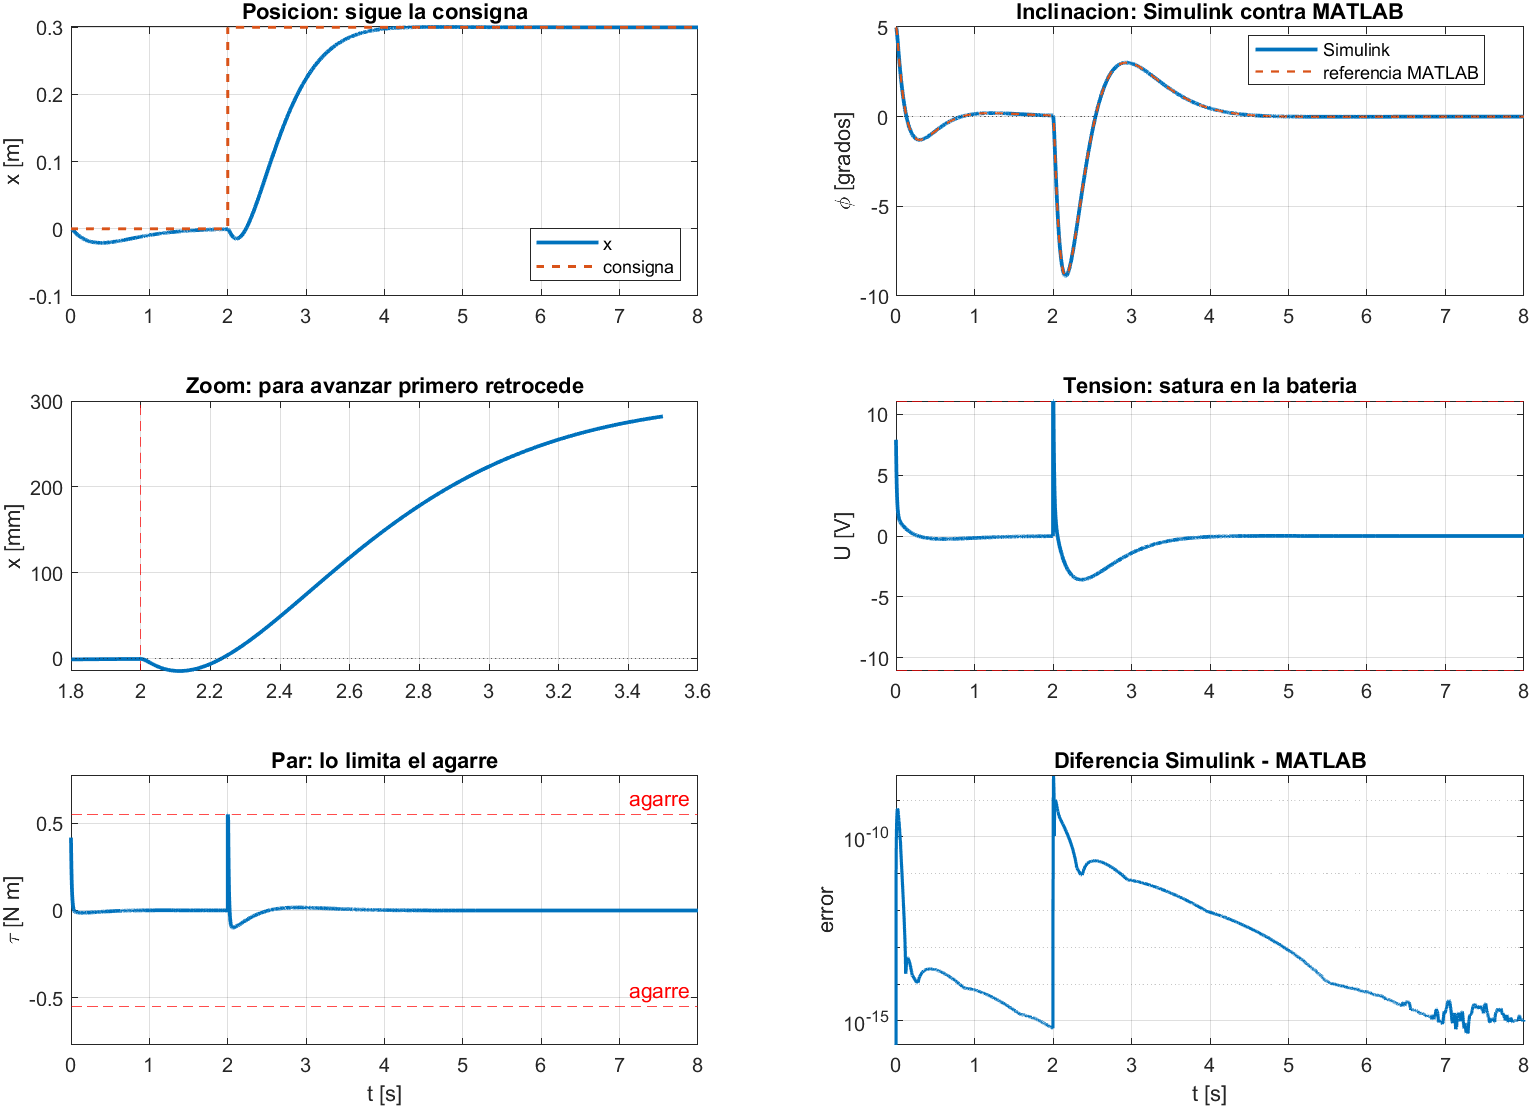
\includegraphics[width=\textwidth]{respuesta_lqr.png}
\captionof{figure}{Las dos cosas que se le piden al robot: quedarse parado y moverse a otra
posición.}
\end{center}

\begin{center}
\begin{tabular}{@{}lr@{}}
\toprule
\multicolumn{2}{@{}l}{\textbf{a) Quedarse parado, arrancando inclinado $5^\circ$}}\\
Inclinación a los 2 s & $0{,}056^\circ$ \\
Cuánto se corrió del lugar & 21{,}4 mm \\
\midrule
\multicolumn{2}{@{}l}{\textbf{b) Ir a 30 cm}}\\
Error final & 0{,}0 mm \\
Retroceso antes de avanzar & 13{,}9 mm \\
Inclinación máxima & $8{,}59^\circ$ \\
Tiempo al 98\% & 1{,}84 s \\
\midrule
\multicolumn{2}{@{}l}{\textbf{Común}}\\
Tensión pico & 11{,}10 V de 11{,}1 \\
Tiempo saturando el agarre & 0\% \\
Normal mínima & 8{,}7 N (la rueda nunca despega) \\
\bottomrule
\end{tabular}
\end{center}

\section{Por qué se puede confiar en el resultado}

Simulink no se valida solo. El mismo problema se integra en paralelo con \texttt{ode45} sobre
una implementación \emph{independiente} de la planta, escrita a mano. Las dos coinciden en:

\begin{center}
\begin{tabular}{@{}lr@{}}
\toprule
$x$ & $2{,}3\times10^{-12}$ m \\
$v$ & $1{,}7\times10^{-10}$ m/s \\
$\varphi$ & $2{,}0\times10^{-11}$ rad \\
$\omega$ & $1{,}5\times10^{-9}$ rad/s \\
\bottomrule
\end{tabular}
\end{center}

Además hay una verificación de seis grupos que corre en los tests: simetría y definición
positiva de $M$, las matrices $A$ y $B$ contra diferencias finitas, el balance de potencia,
el balance horizontal de Newton y la deriva de energía sin fricción. Los seis pasan, y la
suite completa del proyecto está en \textbf{24 de 24}.

% ===========================================================================
\chapter{Qué pasa si las patas se mueven}\label{cap:patasmov}
% ===========================================================================

\begin{idea}
Todo lo anterior congela las patas. Si los dos servos pasan a ser actuadores, la altura del
péndulo cambia mientras el robot se equilibra. La pregunta es si eso rompe el control.
La respuesta corta: \textbf{no}, pero hay que corregir una cosa en el firmware.
\end{idea}

\section{Cuánto cambia la planta}

\begin{center}
\begin{tabular}{@{}rrrrrr@{}}
\toprule
\textbf{Postura} & \textbf{Alto CoM} & \textbf{Brazo $\ell$} & \textbf{Polo} &
\textbf{$\delta_G$} & \textbf{$K_\varphi$} \\
$[^\circ]$ & [cm] & [cm] & [s$^{-1}$] & $[^\circ]$ & \\
\midrule
10 (plegada) & 7{,}2 & 3{,}94 & 7{,}33 & 9{,}09 & $-80{,}0$ \\
15 & 8{,}8 & 5{,}46 & 7{,}54 & 6{,}10 & $-85{,}2$ \\
20 & 10{,}2 & 6{,}86 & 7{,}51 & 4{,}52 & $-89{,}6$ \\
25 & 11{,}5 & 8{,}17 & 7{,}38 & 3{,}58 & $-93{,}5$ \\
30 & 12{,}7 & 9{,}42 & 7{,}23 & 2{,}94 & $-97{,}1$ \\
35 & 13{,}9 & 10{,}62 & 7{,}06 & 2{,}41 & $-100{,}4$ \\
40 (estirada) & 15{,}1 & 11{,}79 & 6{,}89 & 1{,}78 & $-103{,}7$ \\
\bottomrule
\end{tabular}
\end{center}

El centro de masa \textbf{se duplica} en altura, de 7{,}2 a 15{,}1 cm. Y sin embargo el polo
inestable se mueve apenas un 5\%, de 7{,}33 a 6{,}89 s$^{-1}$, con un máximo en el medio.

\begin{idea}
La intuición de la escoba --- cuanto más larga, más fácil de equilibrar --- \textbf{no se
aplica acá}. Esa intuición vale para una masa puntual, donde el polo es $\sqrt{g/\ell}$. En
este robot la \emph{inercia propia del cuerpo} domina sobre el efecto péndulo, y los dos
efectos se compensan.

Dicho de otro modo: \textbf{las patas no sirven para equilibrar}. Sirven para dar despeje,
para amortiguar el aterrizaje (capítulo \ref{cap:din}) y para levantarse.
\end{idea}

\section{¿Hace falta un controlador distinto en cada postura?}

No. Aplicando el $K$ diseñado a $25^\circ$ sobre la planta de cada postura:

\begin{center}
\begin{tabular}{@{}rrrr@{}}
\toprule
\textbf{Postura} & \textbf{Polo lento} & \textbf{¿Estable?} & \textbf{Asentamiento} \\
\midrule
$10^\circ$ & $-1{,}55$ s$^{-1}$ & sí & 2{,}59 s \\
$25^\circ$ & $-2{,}67$ s$^{-1}$ & sí & 1{,}50 s \\
$40^\circ$ & $-2{,}86$ s$^{-1}$ & sí & 1{,}40 s \\
\bottomrule
\end{tabular}
\end{center}

Es estable en todo el rango, con margen de fase entre $85^\circ$ y $96^\circ$. El precio de
usar un solo $K$ es que, con la pata totalmente plegada, el robot tarda un 46\% más en
asentarse. Es un precio barato comparado con la complejidad de programar \emph{gain
scheduling}.

\begin{idea}
\textbf{Recomendación: un solo $K$, el de la postura media.} Si más adelante se quiere afinar,
lo que más se gana es subir $|K_\varphi|$ y $|K_\omega|$ a medida que la pata se estira: de
punta a punta cambian un 30\% y un 47\% respectivamente. Las ganancias de posición y velocidad
no cambian nada.
\end{idea}

\section{Lo que sí hay que corregir}

\begin{ojo}
Mirá la columna $\delta_G$ de la tabla: va de $9{,}09^\circ$ con la pata plegada a
$1{,}78^\circ$ con la pata estirada. $\delta_G$ es lo que hay entre el ángulo del chasis ---
que es lo que mide la IMU --- y $\varphi$, que es lo que necesita el control.

O sea: \textbf{al mover la pata, el cero del ángulo se corre $7{,}31^\circ$}. Si el firmware
no lo corrige, el control va a creer que el robot está inclinado cuando no lo está.
\end{ojo}

Simulado con la planta no lineal, estirando la pata de $10^\circ$ a $40^\circ$:

\begin{center}
\begin{tabular}{@{}lrr@{}}
\toprule
& \textbf{Se corre} & \textbf{Inclinación máxima} \\
\midrule
Sin compensar & 215 mm & $1{,}0^\circ$ \\
\textbf{Compensando} & \textbf{0 mm} & \textbf{$0{,}0^\circ$} \\
\bottomrule
\end{tabular}
\end{center}

No se cae en ninguno de los dos casos --- el robot aguanta ---, pero sin compensar se corre
21 cm del lugar cada vez que cambia de postura. La corrección es una línea:

\begin{center}
\texttt{phi = angulo\_imu + delta\_G(postura\_del\_servo)}
\end{center}

y $\delta_G$ es una función conocida de la postura, que el servo ya sabe porque es él quien la
comanda. Se tabula una vez y se interpola.

\begin{ojo}
Esta simulación interpola los coeficientes de la planta entre posturas. Es una aproximación:
el modelo exacto con patas móviles necesita $\theta$ como tercera coordenada del estado, y
ese modelo todavía no está hecho. Lo que sí es exacto es la tabla de la sección anterior,
porque cada fila es un modelo congelado completo. En otras palabras: \emph{que las ganancias
casi no cambian} está firme; \emph{que cuesta 21 cm} es una estimación.
\end{ojo}

% ===========================================================================
\chapter{Lo que falta medir}\label{cap:falta}
% ===========================================================================

\begin{idea}
El modelo está cerrado y verificado, pero descansa sobre un puñado de números que nadie midió.
Este capítulo dice cuáles son y cuánto cambiaría la conclusión si estuvieran mal.
\end{idea}

\begin{center}
\small
\begin{tabular}{@{}llp{7.0cm}@{}}
\toprule
\textbf{\#} & \textbf{Qué} & \textbf{Si está mal, cambia\ldots} \\
\midrule
M-1 & $\mu$ del neumático & \textbf{todo el margen de tracción}. Es el único parámetro
sin ninguna cota \\
M-6 & rigidez del neumático & \textbf{todo el pico del golpe al aterrizar} \\
M-2 & par real y rendimiento del reductor & el par disponible $\pm25\%$ \\
M-3 & resolución del encoder & el filtro de velocidad y el ruido que entra al control \\
M-4 & masa de rueda y motor & el brazo $\ell$ y el polo inestable ($\pm5\%$) \\
M-5 & inercia del rotor & el coeficiente de avance, hasta un 43\% \\
\bottomrule
\end{tabular}
\end{center}

\section{Por qué el diseño igual es robusto}

Se movió cada suposición una por una. El polo inestable se queda entre 7{,}38 y 7{,}83
s$^{-1}$ y la ganancia $K_\varphi$ varía menos de $\pm5\%$ frente a \textbf{todas} las demás
suposiciones juntas.

\textbf{Lo único realmente indeterminado es si patina o no.} Y ahí la buena noticia es que el
equilibrio normal --- inclinarse dos o tres grados --- pide apenas $\mu = 0{,}20$, que lo da
hasta un piso encerado. Recuperarse de $5^\circ$ pide 0{,}50 y de $10^\circ$, 0{,}69.

\begin{idea}
Perder agarre \textbf{no voltea al robot}: le baja la aceleración máxima y la tolerancia a
empujones. Por eso se puede armar y probar el equilibrio sin saber $\mu$, y medirlo después.
\end{idea}

\section{Cómo se mide $\mu$}

\begin{center}
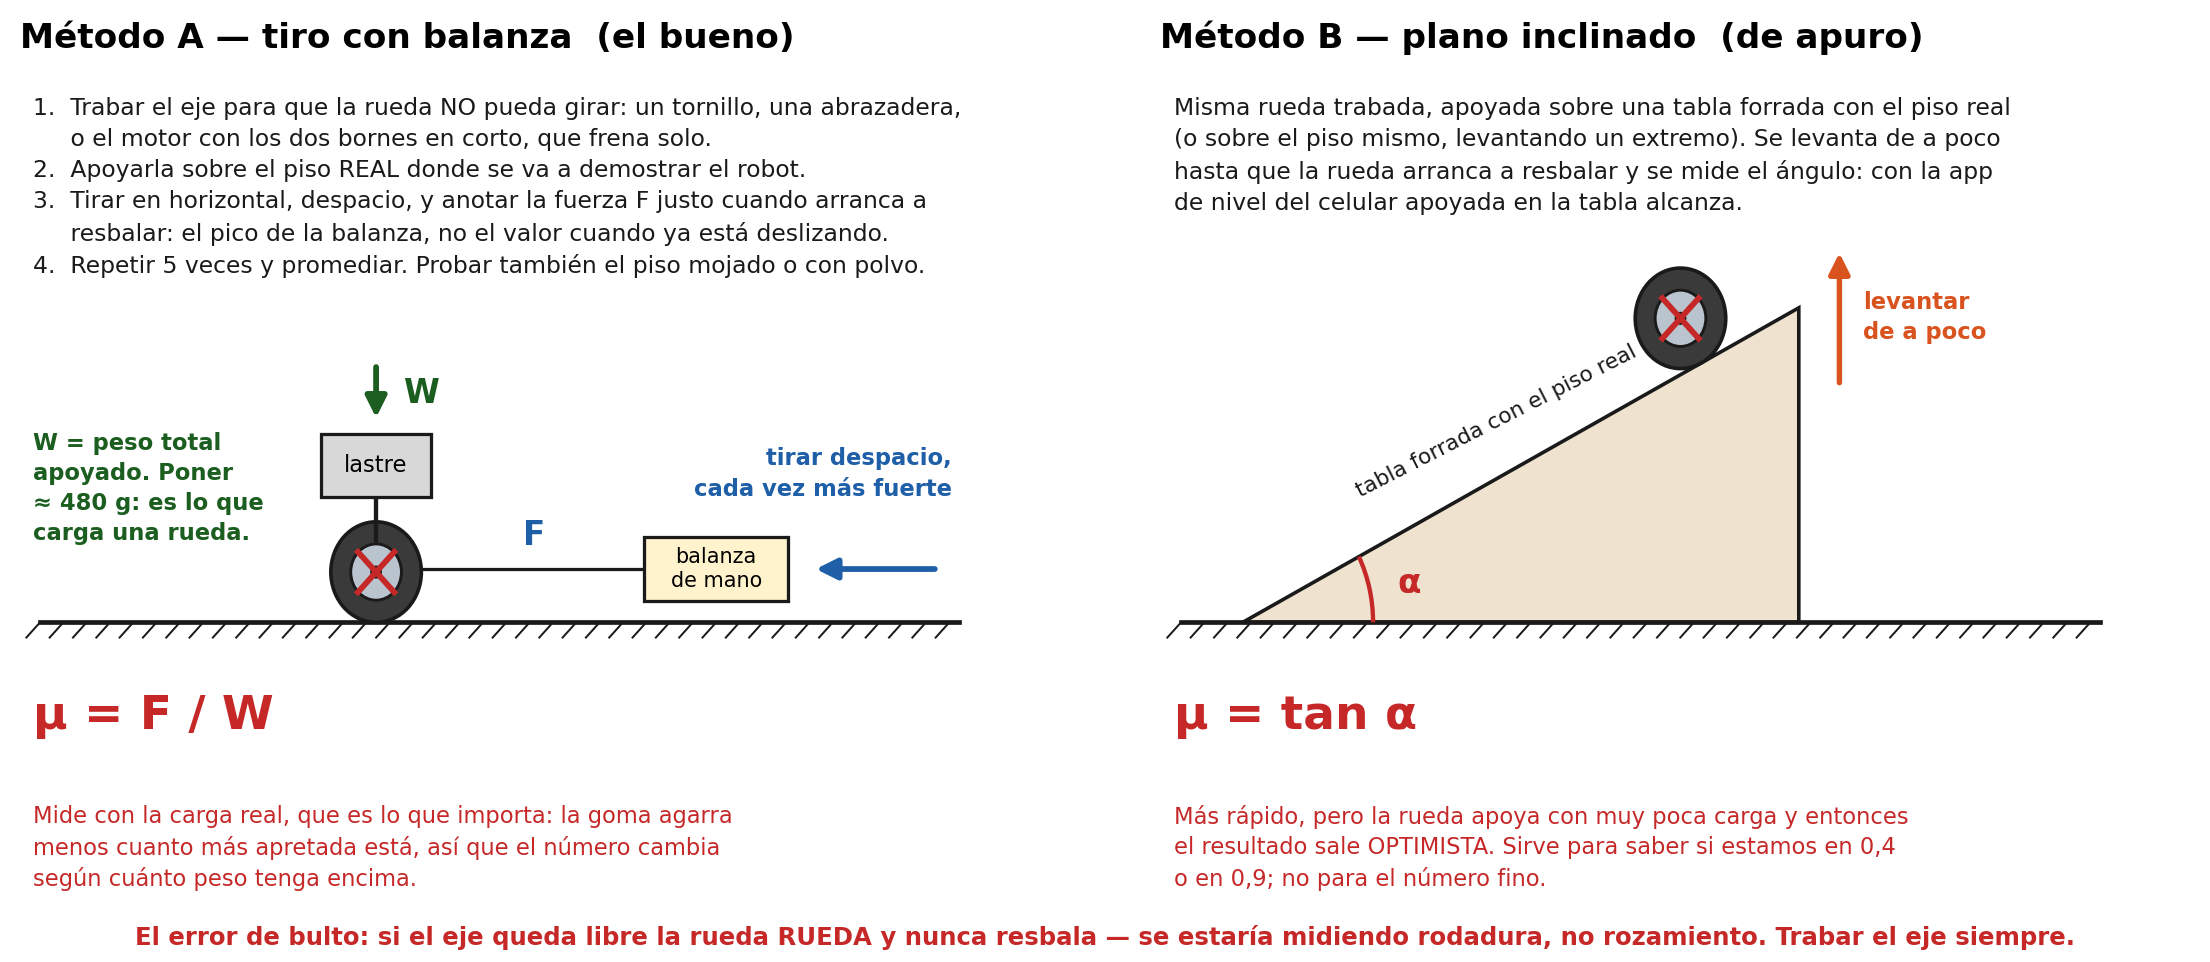
\includegraphics[width=\textwidth]{fig_ensayo_mu.png}
\captionof{figure}{Los dos métodos. Alcanza con una rueda sola: no hace falta el robot
armado.}
\end{center}

El plan completo de ensayos, con los seis y en qué orden hacerlos, está en
\texttt{docs/gestion/2026-10-21-plan-de-ensayos.md}.

% ===========================================================================
\appendix
\chapter{Cinemática de la pata: desarrollo completo}\label{ap:cin}
% ===========================================================================
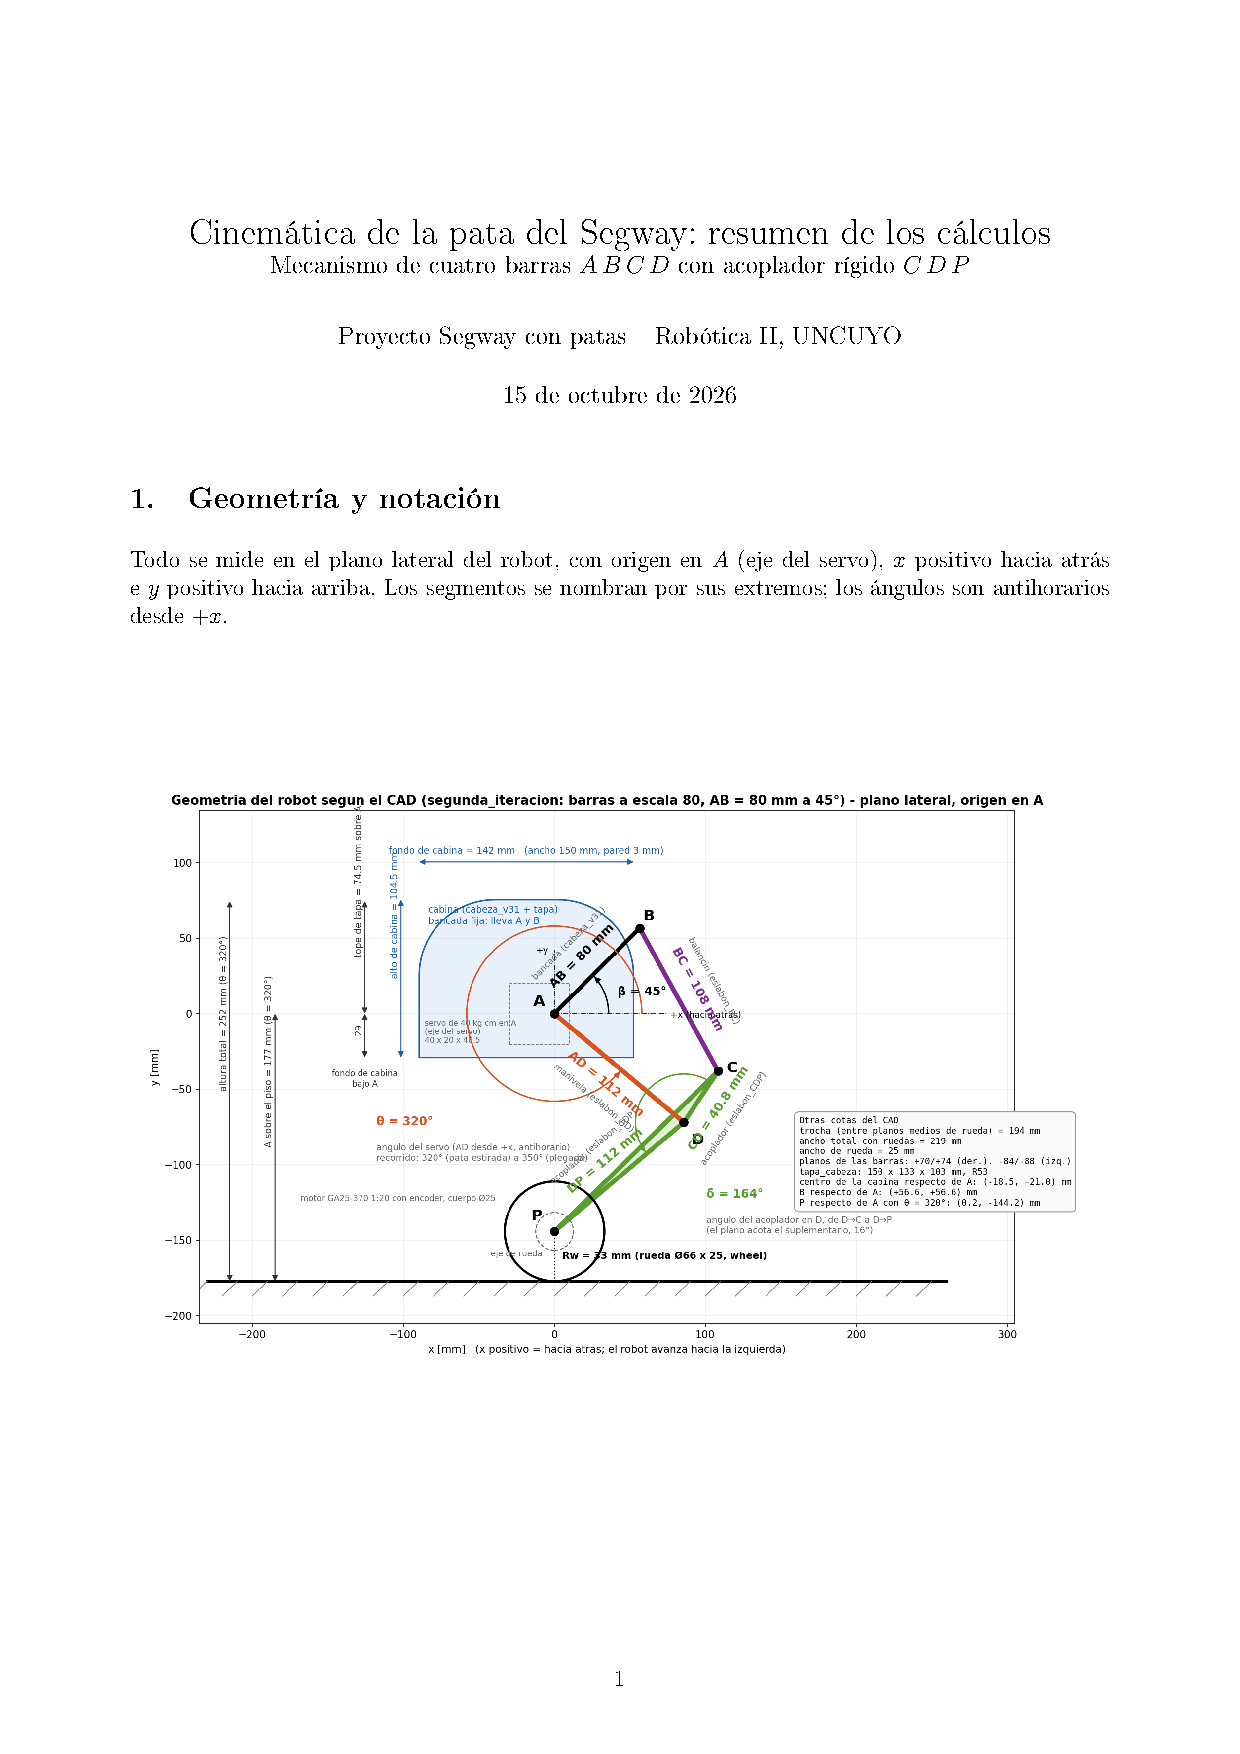
\includepdf[pages=-,scale=0.92,pagecommand={}]{../../modelado/cinematica/cinematica_resumen.pdf}

\chapter{Diagramas de cuerpo libre}\label{ap:dcl}
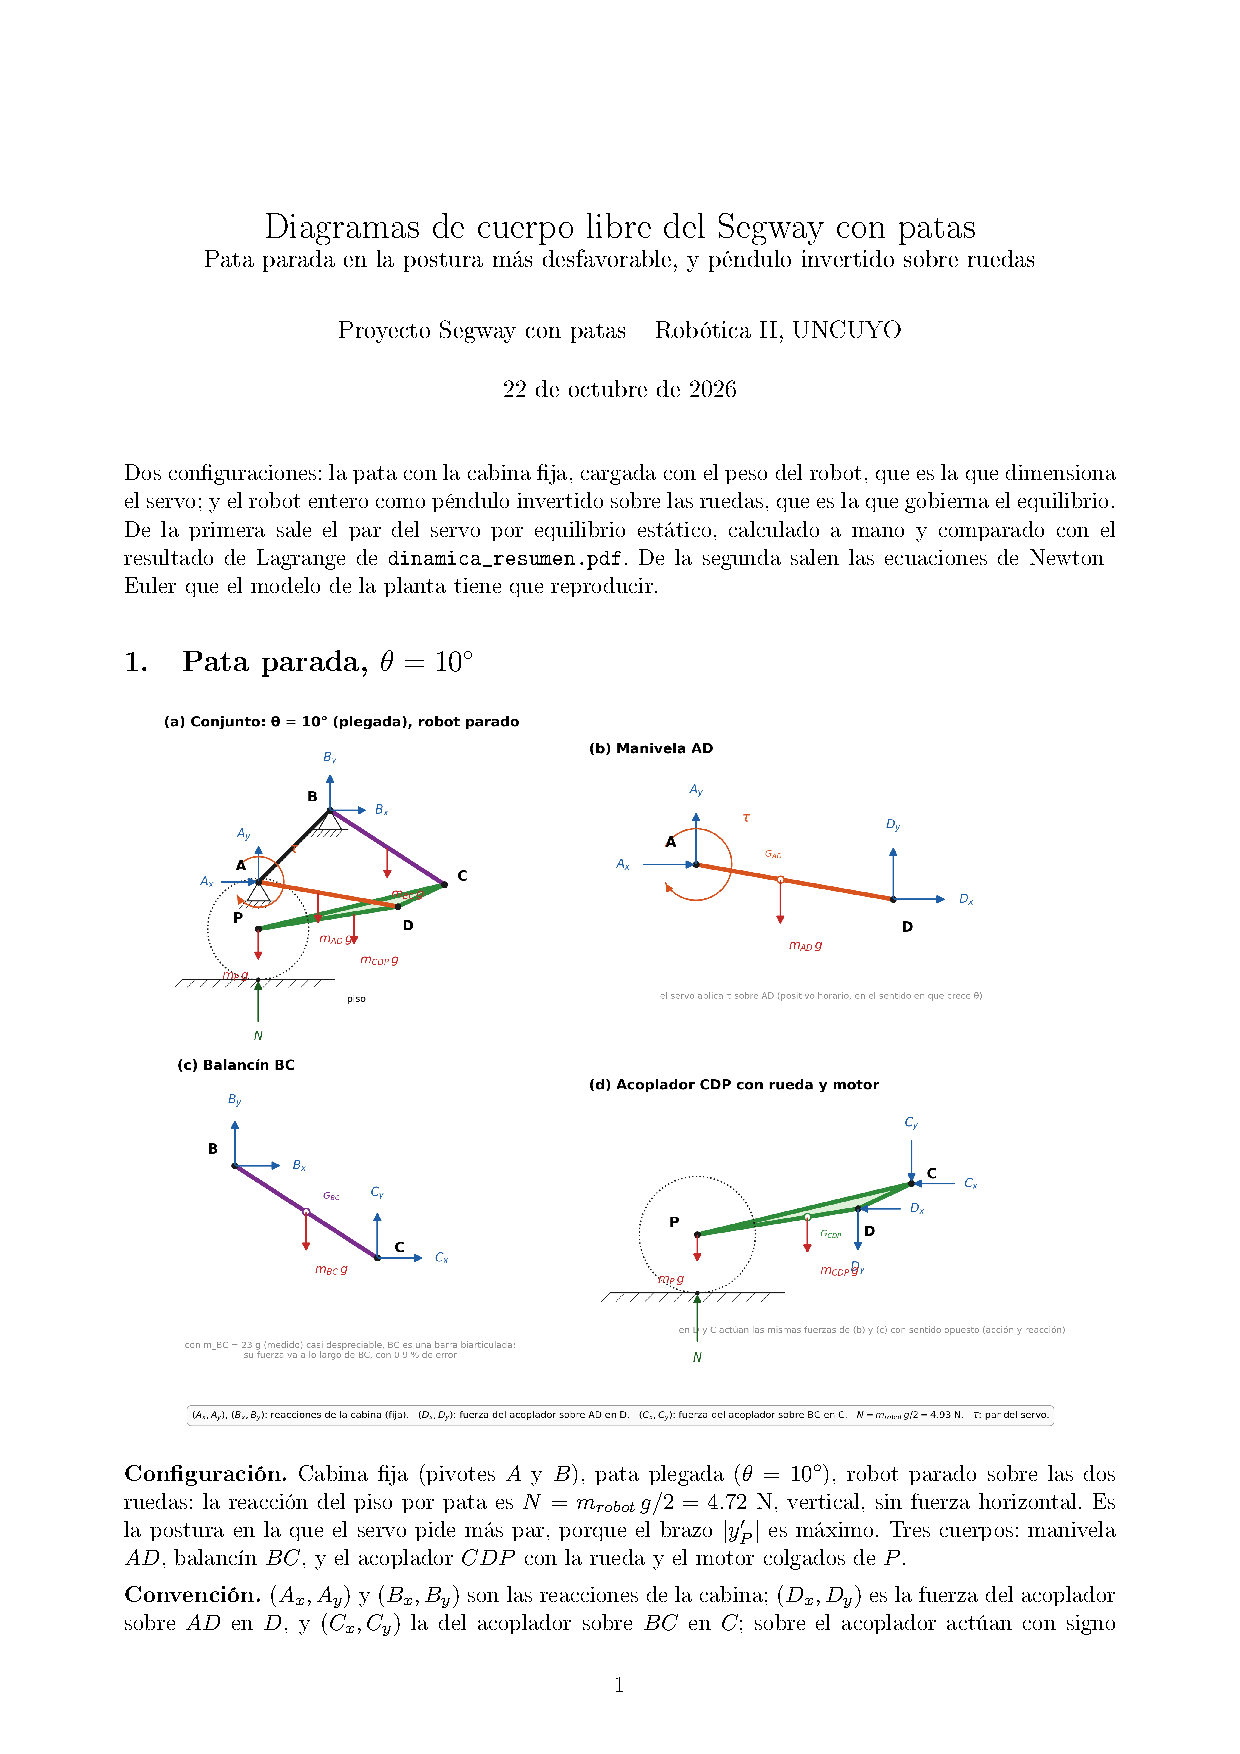
\includepdf[pages=-,scale=0.92,pagecommand={}]{../../modelado/dcl/dcl_resumen.pdf}

\chapter{Dinámica de la pata por Lagrange}\label{ap:dinres}
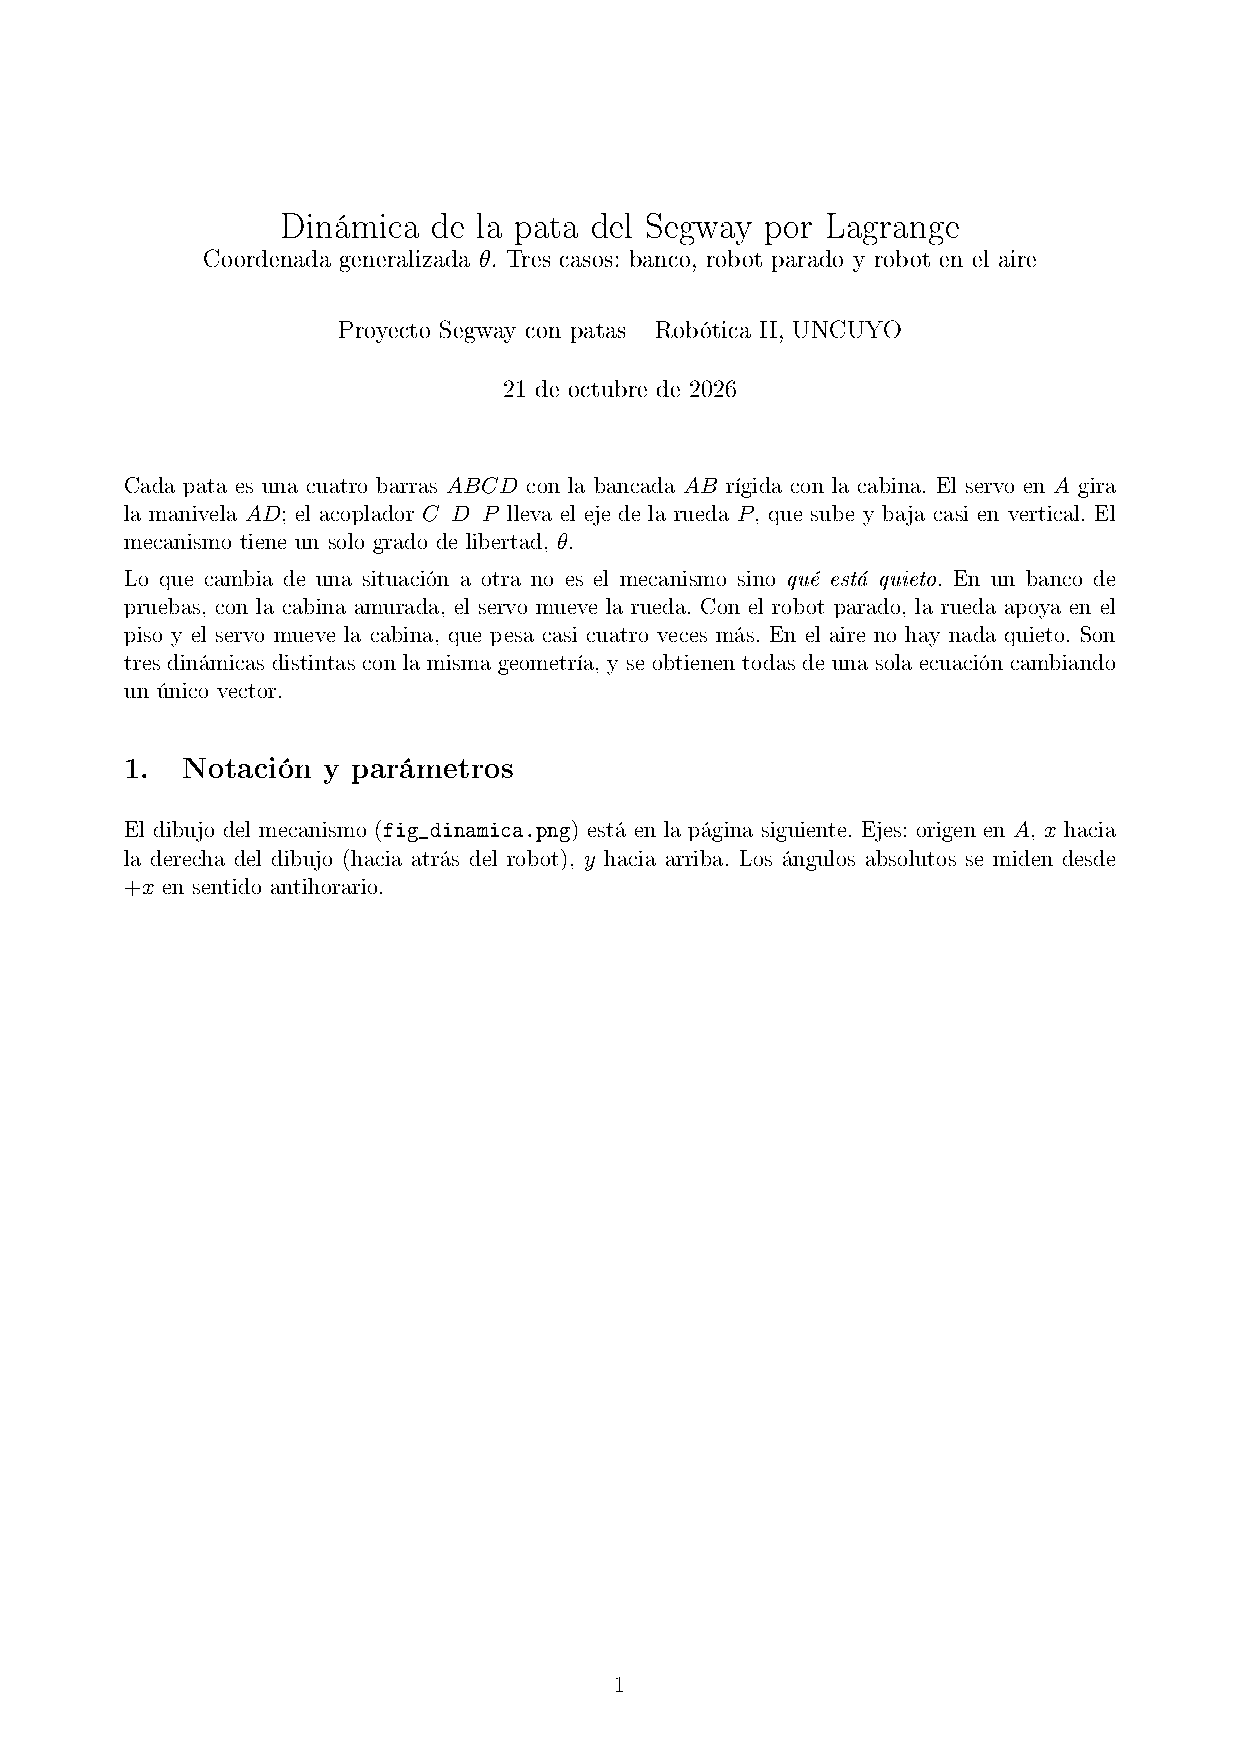
\includepdf[pages=-,scale=0.92,pagecommand={}]{../../modelado/dinamica/dinamica_resumen.pdf}

\chapter{Dinámica de la pata con el robot apoyado}\label{ap:dinapo}
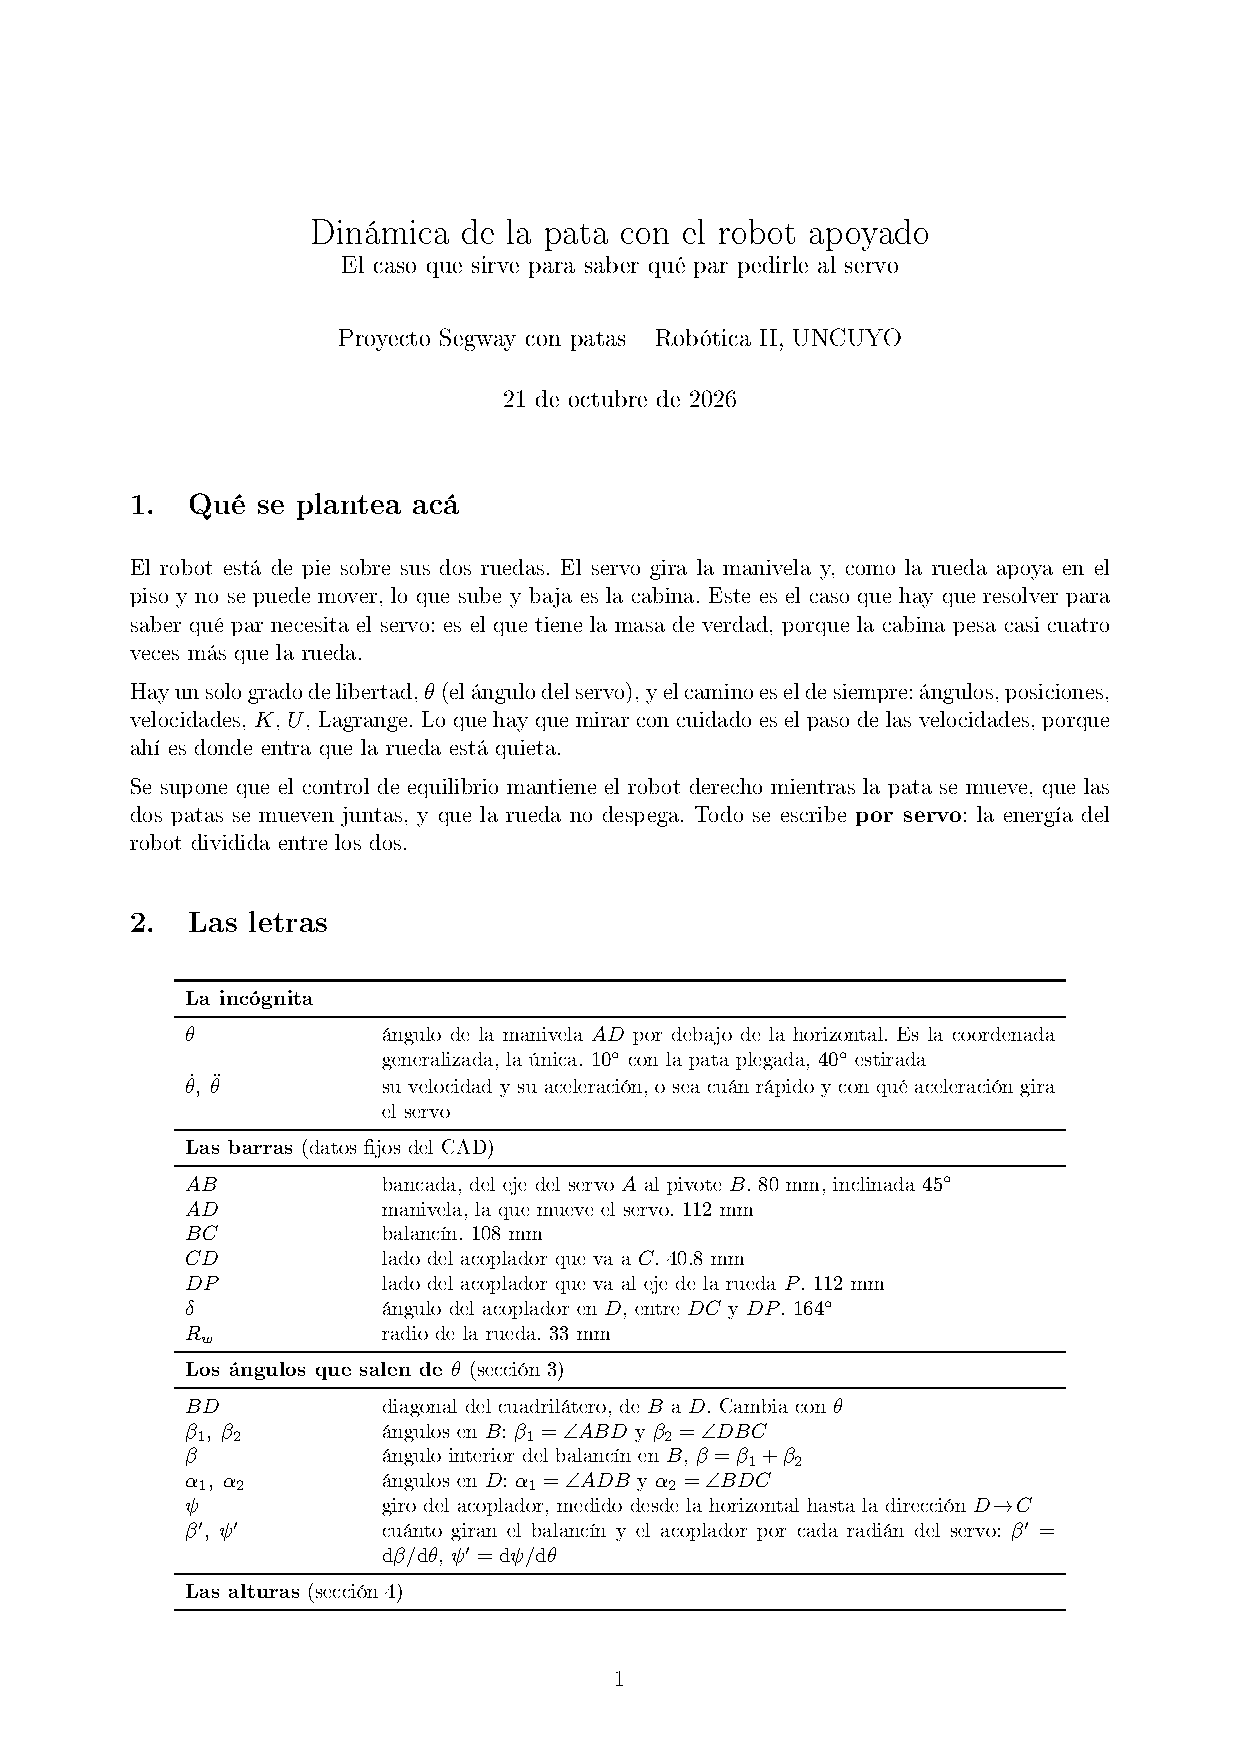
\includepdf[pages=-,scale=0.92,pagecommand={}]{../../modelado/dinamica/dinamica_apoyado.pdf}

\end{document}
